\chapter{Event Reconstruction} \label{chapter:reconstruction}

    \section{Introduction}

        Once a bunch-crossing event has cleared the Level 1 Trigger system, the process of event reconstruction begins.
        An event in ATLAS is initially nothing but a collection of electrical signals collected from the various detectors.
        Event reconstruction is when the myriad detector readings are aggregated together into meaningful patterns,
            which are interpreted as physical objects and physics processes.
        The key objects of interest in this analysis are particle \textit{tracks} and \textit{jets}.
        As well, the way in which b-quark-initiated jets (``b-jets'') are distinguished from other jet types,
            a process called \textit{flavor tagging}, plays a particularly important role.
        Finally, special attention will be given to the fact that reconstruction occurs not once, but twice;
            first in the High Level Trigger online running environment
            and again in the offline environment after events have been moved to permanent storage.
        Though the two iterations are very similar, it is worth discussing how they differ.

    \FloatBarrier
    \section{Tracks} \label{sec:reco_tracks}
            
        \subsection{Track Definition}
            
            The first point of contact for anything leaving the IR of ATLAS is the tracking detectors.
            As such, the objects reconstructed from the tracking detectors will be the first point of discussion.
            Prior to encountering the ATLAS calorimeters,
                particles exiting the IR pass through primarily low-density material (see Fig. \ref{fig:cal_rad_length}).
            Thanks to the inclusion of the solenoid magnet field encompassing the Inner Detectors,
                these trajectories reveal crucial information about the particles in an event.
            This is because any charged particle with a momentum component orthogonal to a magnetic field
                will trace out a \textit{helical} trajectory.
            If the shape of the helix is known, then basic electrodynamics principles can be used to determine the
                momentum and charge of the originating particle.
            Specifically, for a charged particle with four-momentum given as 
            \begin{equation}
            p = \minimatrix{E \\ p_T \\ \theta \\ \phi}
            \end{equation}
            the track's helical shape can reveal all components except for the energy $E$,
                which may eventually be determined from the calorimeters/muon system.
            To understand how this is achieved, one must understand how a track helix is described mathematically.
            A helix can be defined using five parameters structured in a three-dimensional parametric equation\cite{thesis_giacinto}.
            There are several conventions for the form these parameters should take,
                but in ATLAS a helix is described by a set of equations parameterised by an angle $\alpha$ as:
            \begin{equation} \begin{split}
                x(\alpha) &= x_R + d_0 \cos(\phi) + r \left[ \cos(\alpha) - \cos(\phi) \right] \\
                y(\alpha) &= y_R + d_0 \sin(\phi) + r \left[ \sin(\alpha) - \sin(\phi) \right] \\
                z(\alpha) &= z_R + z_0 - r \cot(\theta) (\alpha - \phi)
                \,.
            \end{split} \end{equation}

            The helix is described relative to a reference point $R$,
                which is initially set to the beam-spot location in the IR.
            Later stages of tracking will redefine the equations with respect to different reference points as needed.
            The five parameters governing the shape of this helix,
                called \textit{perigee parameters} (see Figs. \ref{fig:perigee_params_base}-\ref{fig:perigee_params_top}),
                are described largely in terms of the ``Point of Closest Approach'' (PoCA),
                the point on the helix closest to $R$ in the $x,y$ plane.
            These perigee parameters are the following:
            \begin{itemize}
                \item $d_0$: $|(x,y)|$-distance from the origin to the closest point on the helix, in the $x,y$ plane
                \item $z_0$: $z$-distance between the PoCA and the origin
                \item $\phi$: Angle in the $x,y$ plane of the PoCA
                \item $r$: The radius of curvature of the helix
                \item $\theta$: The angle of the helix's trajectory in the $r,z$ plane
            \end{itemize}

            \begin{figure}[tbh]
                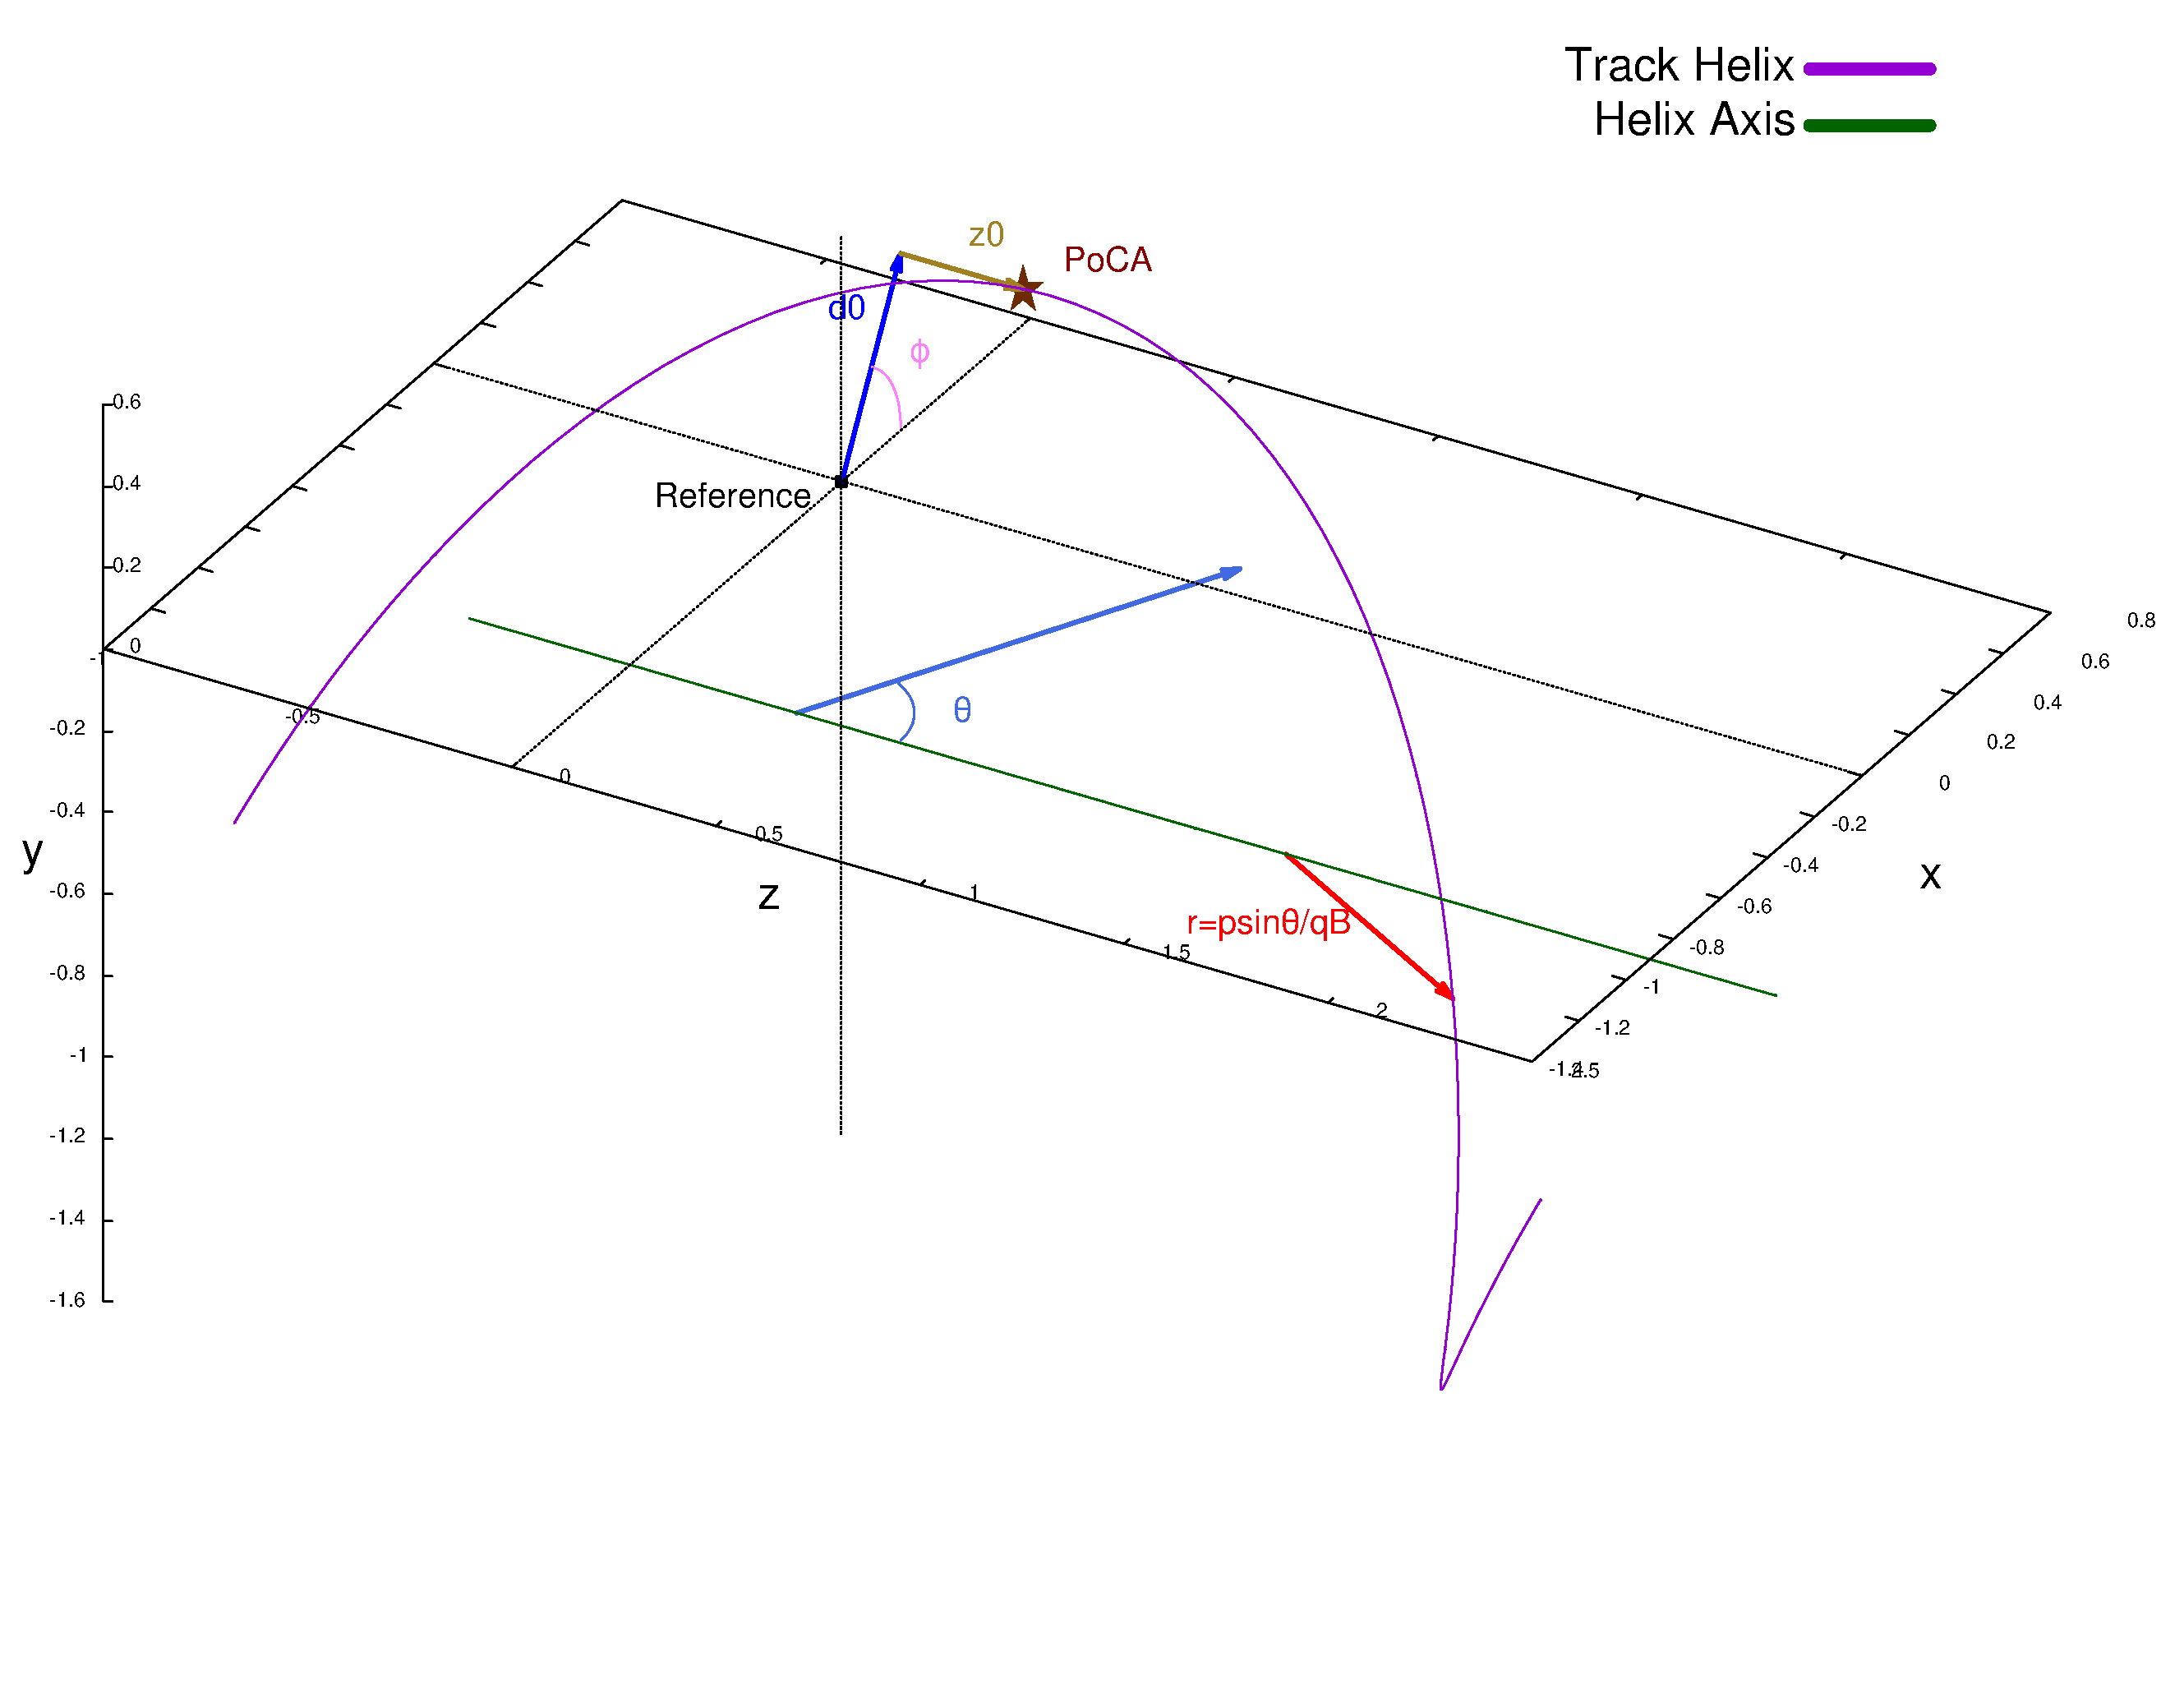
\includegraphics[width=\linewidth,height=\textheight,keepaspectratio]{reconstruction/perigee_base}
                \caption{
                    A diagram showing a helix trajectory from an isometric perspective,
                        with the five perigee parameters highlighted.
                    The interactive 3D form of this plot can be accessed by running Gnuplot\cite{gnuplot} on this script:
                        \url{https://github.com/cmilke/phd_thesis/blob/master/scripts/perigee_plot.gp}.
                }
                \label{fig:perigee_params_base}
            \end{figure}

            \begin{figure}[tbh]
                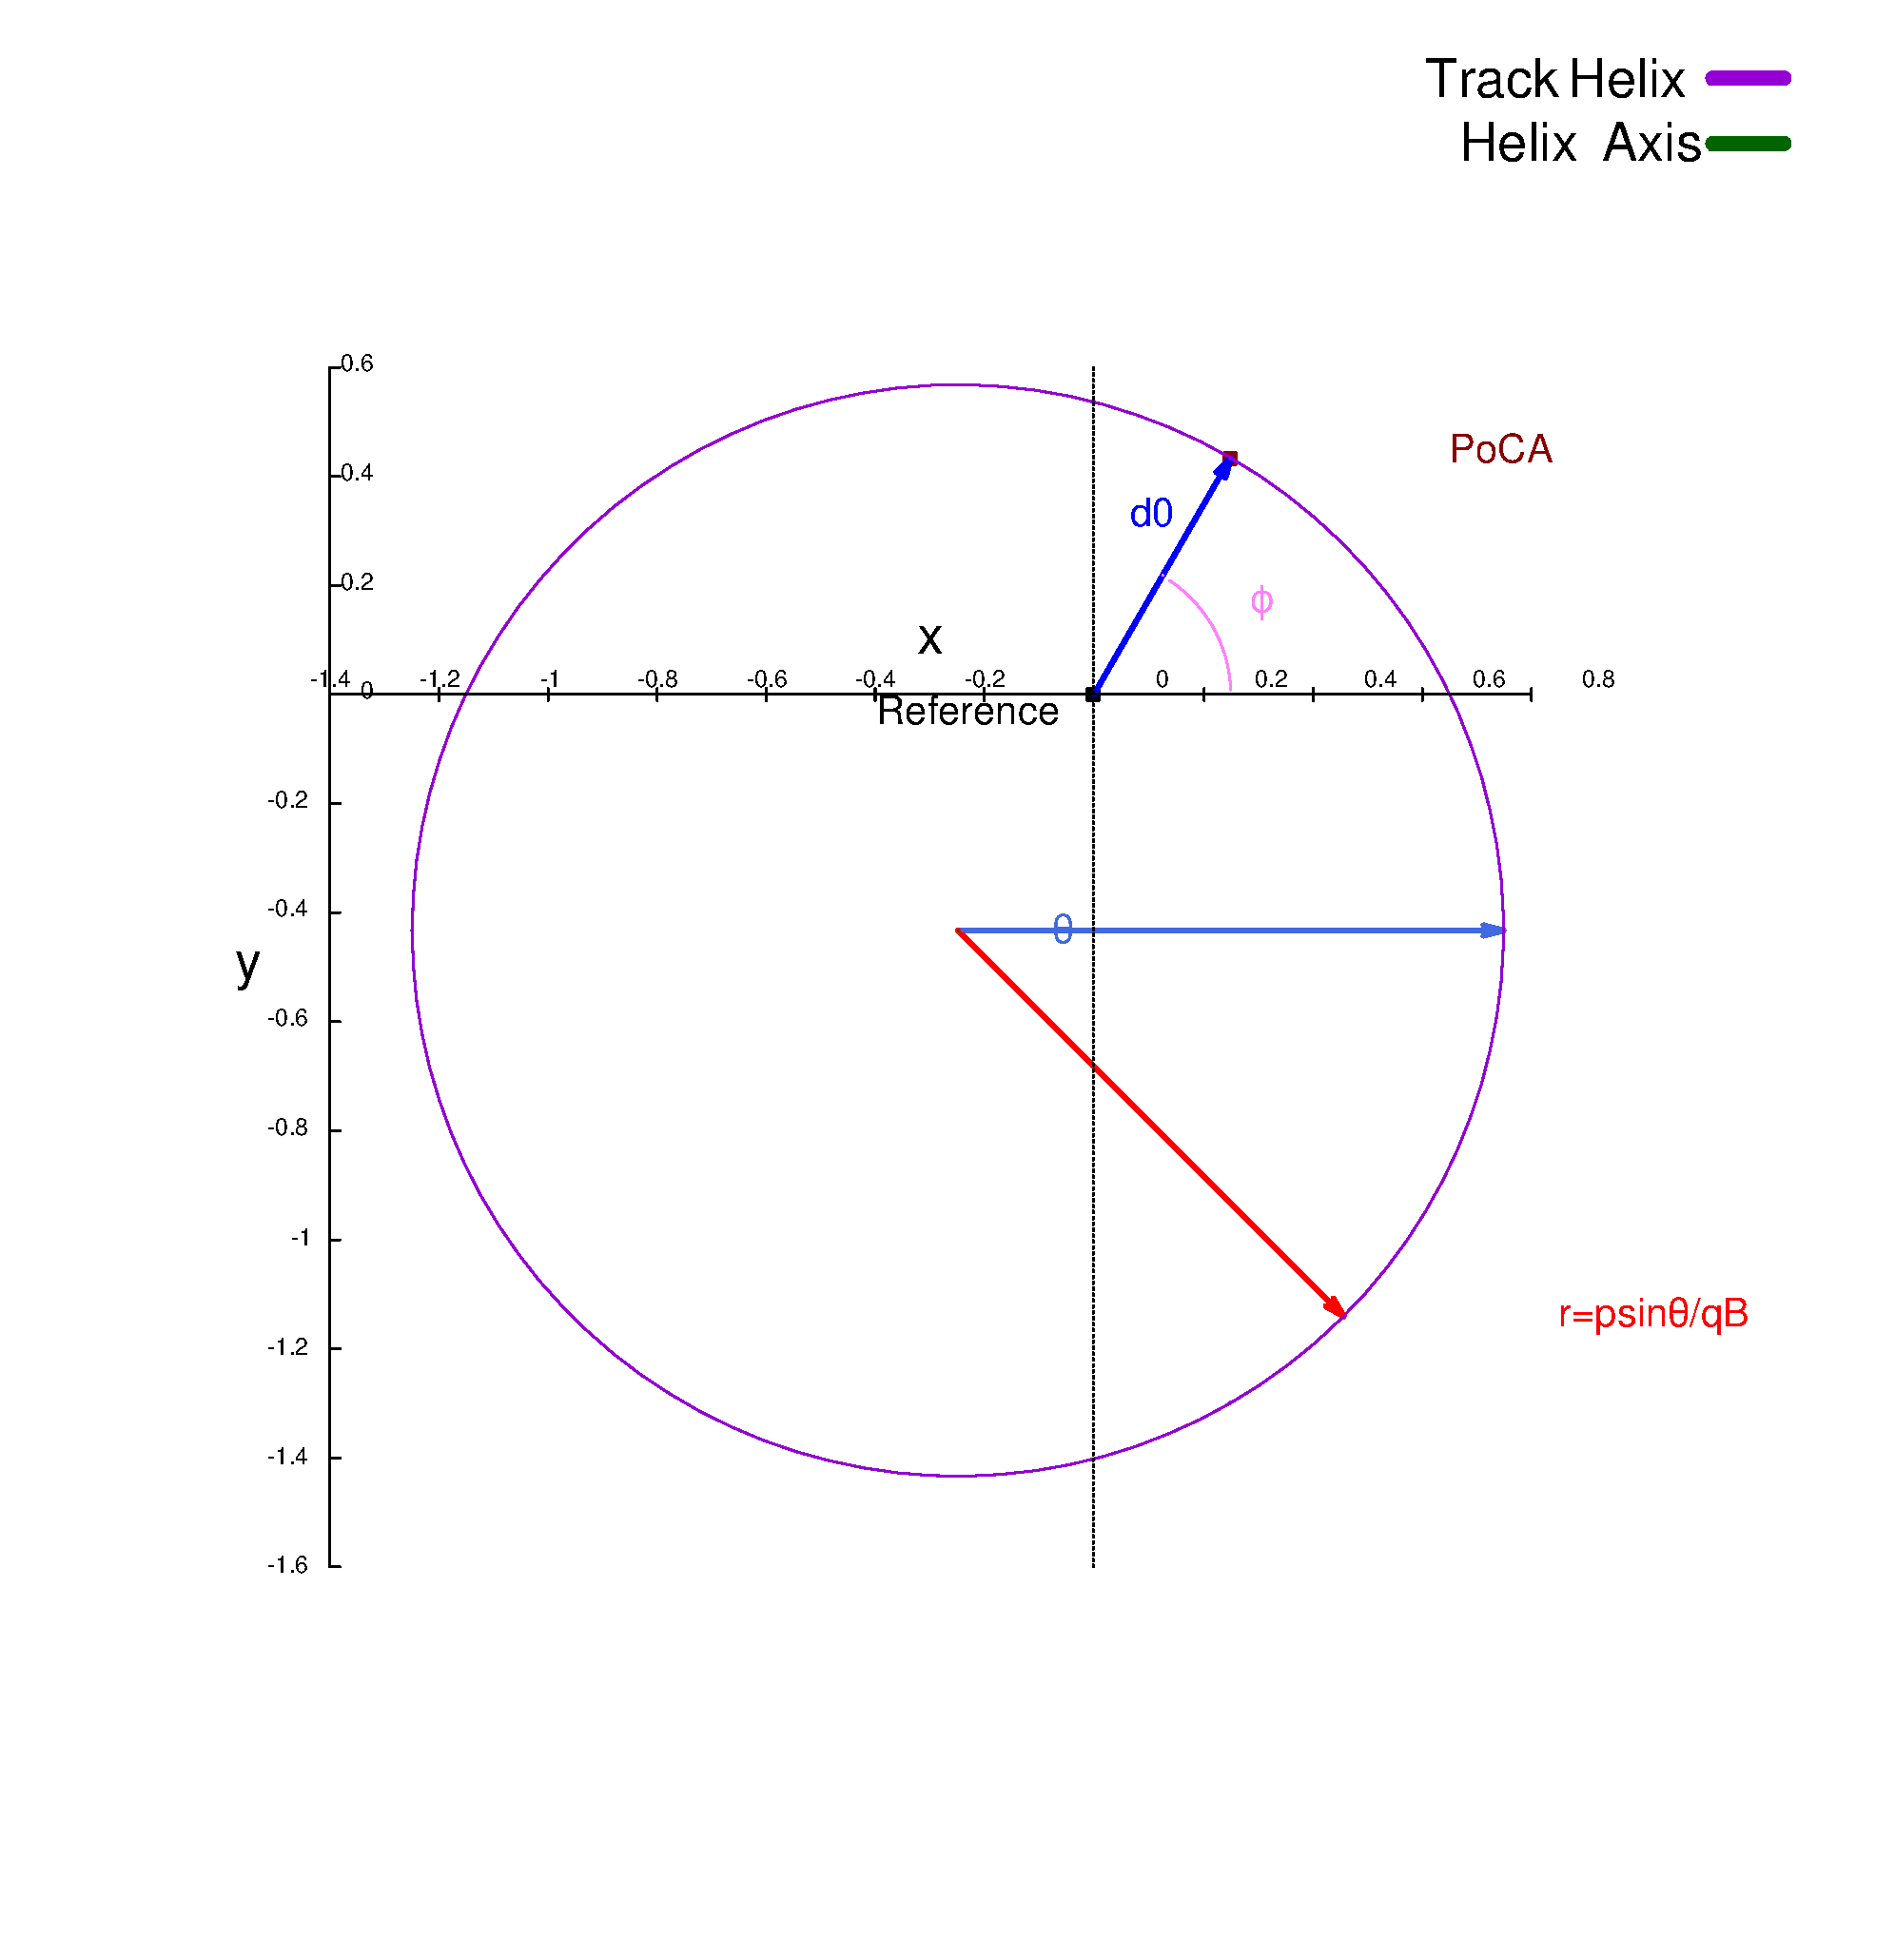
\includegraphics[width=\linewidth,height=\textheight,keepaspectratio]{reconstruction/perigee_front}
                \caption{
                    A diagram showing a helix trajectory, looking down the beampipe (z),
                        with the five perigee parameters highlighted.
                }
                \label{fig:perigee_params_front}
            \end{figure}

            \begin{figure}[tbh]
                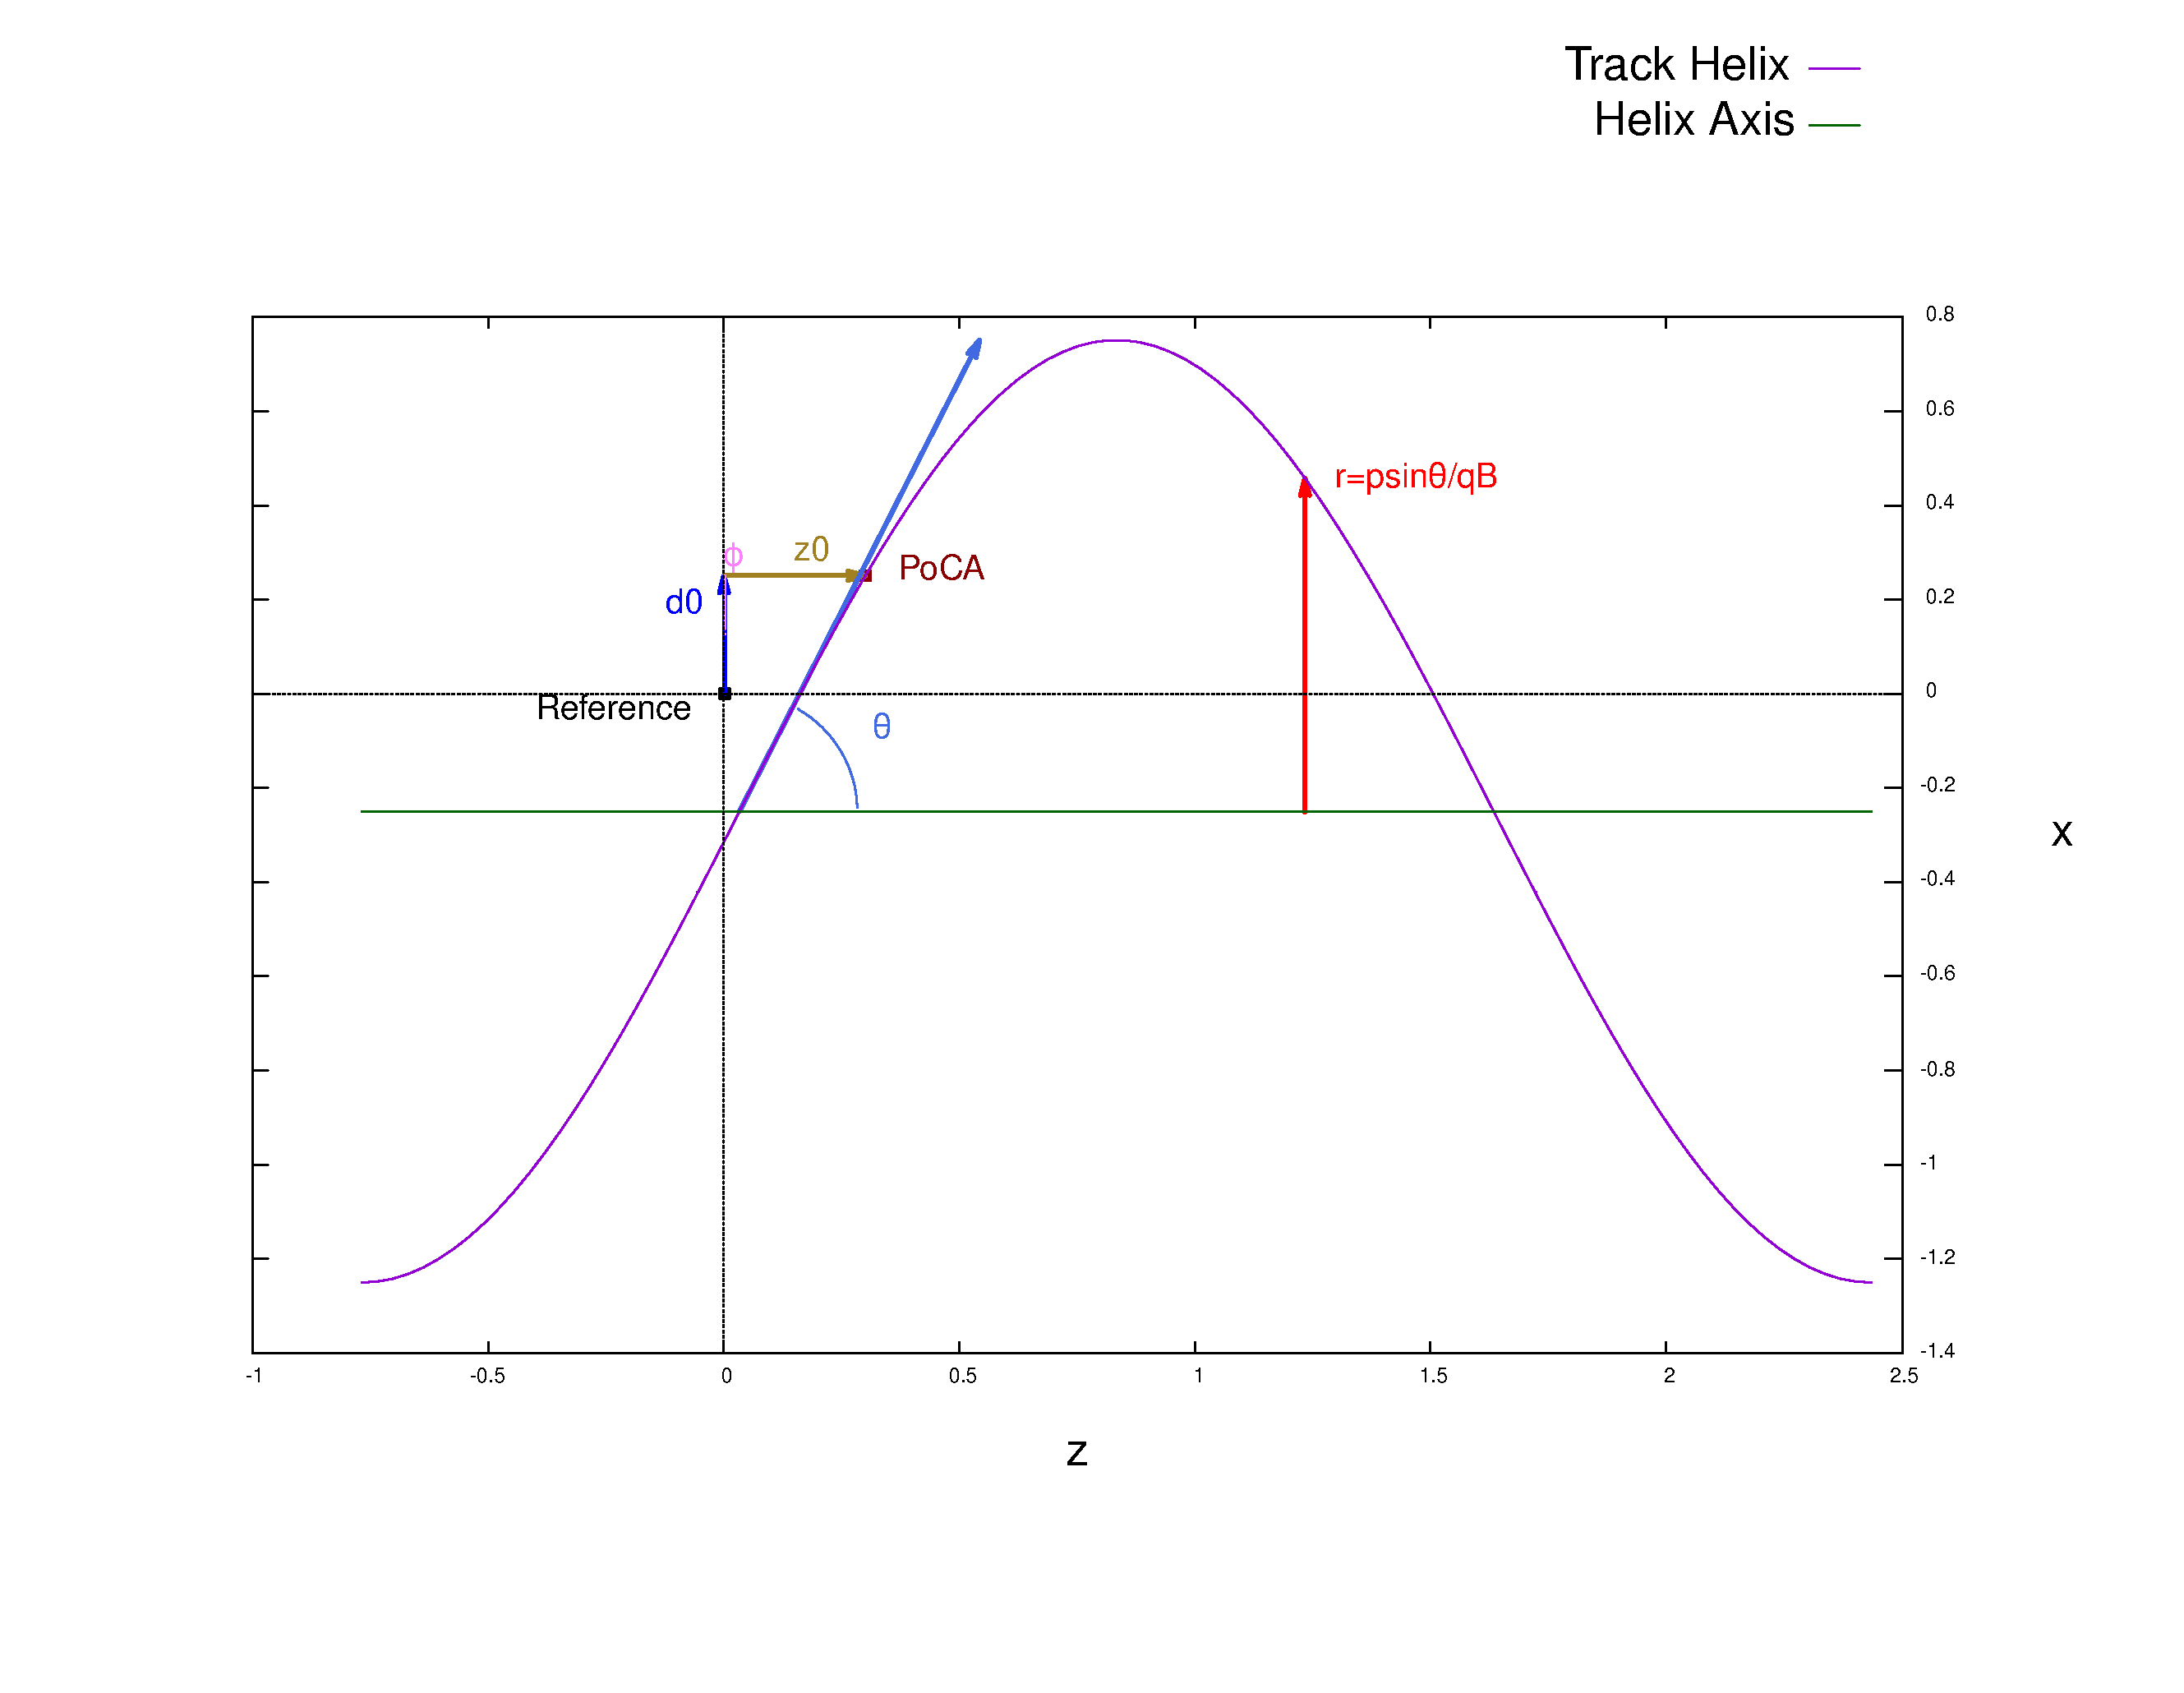
\includegraphics[width=\linewidth,height=\textheight,keepaspectratio]{reconstruction/perigee_top}
                \caption{
                    A diagram showing a helix trajectory from a top-down perspective,
                        with the five perigee parameters highlighted.
                }
                \label{fig:perigee_params_top}
            \end{figure}

            All five of the parameters are used at some stage of the analysis.
            With regards to the particle momentum, $\phi$ and $\theta$ are themselves components of the particle's 4-vector.
            $r$ can be related to the particle's transverse momentum and electric charge by:
            \begin{equation}
                r = \frac{p_T}{qB} = \frac{|\vec{p}| \sin \theta}{qB}
            \end{equation}
            where $B$ is the magnetic field\footnote{
                    Note that this equation only really works for a perfectly uniform axial field.
                    In practice the calculations are performed using a magnetic field vector map.
                } of the Inner Detector Solenoid Magnet\cite{thesis_track_sim_and_reco}.
            %Note that uncharged particles (e.g.\ photons) will not be bent, and so will have no curvature,
            %    negating the ability to measure their transverse momentum in this way.
            The impact parameters, $d_0$ and $z_0$, are not related to momentum,
                but will be used in later sections for the purpose of flavor tagging.

        \subsection{Track Reconstruction}

            As particles pass through the inner detector subsystems, they trace out a path in ionized detector elements.
            This trajectory can be reconstructed by effectively playing connect-the-dots.

            %Clusterization
            The first step in reconstructing a track is to determine the points at which a track traversed detector elements,
                a process called ``clusterization''\cite{atlas_track_reco_performance}.
            Ionizing particles often deposit energy across several adjacent pixels on a given layer.
            A \textit{connected component analysis} algorithm\cite{connected_component_analysis}
                is used to group pixels together.
            Based on the pattern of energy distribution in these groups,
                a \textit{space-point} (the ``dot'' in my metaphor) 
                is created indicating the estimated position at which a particle crossed the detector element.
            Several space-points can be assigned to the same pixel cluster
                if the energy readout pattern suggests multiple particles traversed the same location.

            \begin{figure}[tbh]
                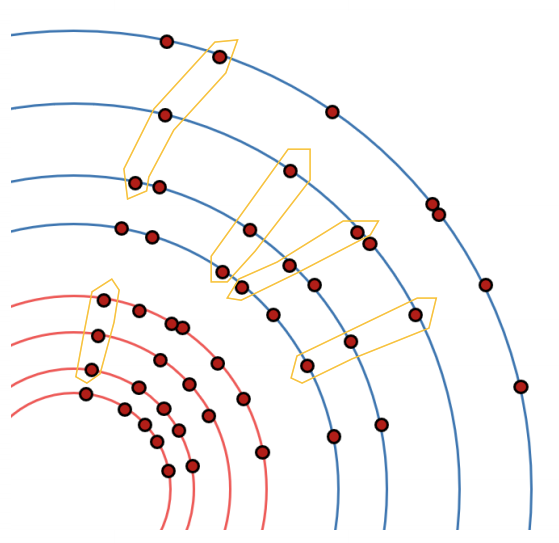
\includegraphics[width=\linewidth,height=\textheight,keepaspectratio]{reconstruction/trackseeding}
                \caption{
                    Diagram of space-points formed in the ATLAS Pixel (Red) and SCT (Blue) subdetectors,
                        with track seeds highlighted in yellow\cite{track_seeding}.
                    Track seeds are formed using ``adjacent'' space-points, in the sense that they
                        occur in sequential detector layers at roughly the same angle in $\eta$ and $\phi$.
                }
                \label{fig:track_fit}
            \end{figure}

            %Combinatorial track finding
            Once the ``dots'' are established, a series of guesses at how they should be connected are made.
            Initial guesses at tracks, called \textit{track seeds},
                are formed by assembling adjacent (see Fig. \ref{fig:track_fit}) combinations of three space-points.
            The number of seeds is limited by generally only allowing space-points to be part of a single track seed.
            Further purity is ensured by forming track seeds first only from the SCT, then only from the pixel detector,
                and only after allowing mixed-detector seeds from the remaining space-points.
            The track seeds are assigned helix parameters by assuming they travel through a uniform magnetic field,
                allowing rapid estimates of the tracks' momenta.
            These seeds are expanded into \textit{track candidates}
                by including more space-points across additional detectors in the ID using a \textit{Kalman filter}\cite{kalman}.

            %Ambiguity solving; NN clustering; Track fit
            The last step is then to choose a final set of best-quality trajectories.
            This is done using a number of criteria involving
                the track's $p_T$ and $\eta$,
                how many clusters it traversed, 
                whether it shared pixels,
                if the track has any ``holes''\footnote{
                    A track hole is an absence of a space-point in detector material intersected by a track
                    where an interaction would otherwise be expected.
                } and its impact parameters with respect to the PV\cite{atlas_track_reco_performance}.
            Tracks can be outright rejected depending on some of these criteria,
                but are also assigned a score if they satisfy them.
            Higher track scores are attained through the number and type of clusters they pass through,
                as well as through higher track momenta.
            Track scores are penalized by having holes or a poor helix fit ($\chi^2$ fit value).
            These scores are used to resolve ambiguities where multiple tracks are assigned to the same space-points,
                with preference given to higher-scoring candidates.
            Neural networks (see Section \ref{sec:ml_techniques})
                are used to assist in some ambiguity solving situations,
                as well as to help identify clusters with multiple valid tracks.
            Once ambiguities have been resolved and all malformed track candidates removed,
                the remaining tracks are refit using all available information at high-resolution\cite{atlas_track_reco_performance}.

        \subsection{Primary Vertexing}

            Once track filtering has concluded,
                the resultant tracks can be used to identify a key piece of event information, 
                called the \textit{Primary Vertex} (PV).
            When bunches collide in the IR of ATLAS, most of the collisions of a given bunch are fairly low energy.
            Events which clear the L1 trigger however,
                typically do so because of the presence of a hard-scatter interaction\footnote{
                    Characterized as an interaction involving significant momentum transfer between partons.
                }.
            Identifying the location along the beamline at which this hard-scatter interaction occurred is achieved via ``vertex-finding.''
            Points along $z$ from which particles originate are referred to as ``vertices.''
            They are identified in reconstruction by tracing the reconstructed tracks backwards
                and identifying points at which they intersect the $z$-axis.
            All tracks which intersect at the same point are associated to that vertex.
            Most of the vertices are of little interest, and are known as ``pile-up vertices.''
            The PV is the vertex assumed to be the location of the hard-scatter interaction,
                and is identified as a vertex associated with at least two tracks
                and whose tracks possess the largest scalar sum of squared transverse momentum
                    \cite{jet_energy_scale13TeV} \cite{primary_vertex_identification}.
                \begin{equation}
                    p_T^2 \textrm{ sum}  \equiv \sum\limits_{i \in \textrm{tracks}} p_{T,i}^2
                    \,.
                \end{equation}
            Once the primary vertex is identified, the high resolution track fitting step is rerun,
                but now with the reference point $R$ set as the PV instead of the beamspot.


    \FloatBarrier
    \section{Jets}\label{sec:jets}

        \subsection{Cell Clustering}

        Moving beyond the inner tracker and extending into the calorimeters,
            focus shifts from tracks to the objects known as ``jets.''
        Jets are the result of an algorithm meant to associate related reconstructed objects in the detector elements
            in order to produce a more comprehensive representation of the physical behavior of the particles traversing those elements.
        Jet reconstruction encompasses all elements of ATLAS,
            but it begins in the calorimeter system in the form of ``topological clusters.''

        Just as the inner trackers suffer from pile-up vertices that must be filtered,
            so too do the calorimeters suffer from pile-up energy deposits and electronic noise.
        Topo-clusters are the reconstructed structure meant to address the issue of noise in the calorimeters
            by emphasizing regions with a high energy-to-noise ratio.
        As such, cell clustering is based on a ``signal-significance'' metric,
            \begin{equation}
                \xi^{\textrm{EM}}_{\textrm{cell}} \equiv \frac{
                    E^{\textrm{EM}}_{\textrm{cell}} }{
                    \sigma^{\textrm{EM}}_{\textrm{noise, cell}} } \,,
            \end{equation}
            where $E^{\textrm{EM}}_{\textrm{cell}}$ is the energy of an individual cell calibrated to the electromagnetic scale
            (see Section \ref{sec:jet_calibration}).
        $\sigma^{\textrm{EM}}_{\textrm{noise, cell}}$ is the noise factor of that cell, calculated for that particular LHC run.

        Clusters start as seeds consisting of just a single high significance cell
            and then follow a collection algorithm described in \cite{cell_clustering} to aggregate nearby cells.
        This collection is performed in three-dimensions, so topo-clusters can occupy multiple layers of a calorimeter.
        The result of the collection algorithm is a ``proto-cluster.''
        Proto-clusters themselves can often be too large to permit analysis of the particles that formed them,
            hence the final step of ``splitting'' them.
        Local signal-significance maxima are identified within the proto-clusters,
            and the collected cells are split between those maxima via another algorithm
            which weights cells per their energy and distance from the local maxima.
        Topo-clusters are the final product of splitting.
        By themselves, topo-clusters do not necessarily correspond to any physical process,
            as they are not necessarily intended to capture the entire response of a particle
            (although they often do).
        Representing the full detector response to a particle is the role of jets.

        \begin{figure}[tbh]
            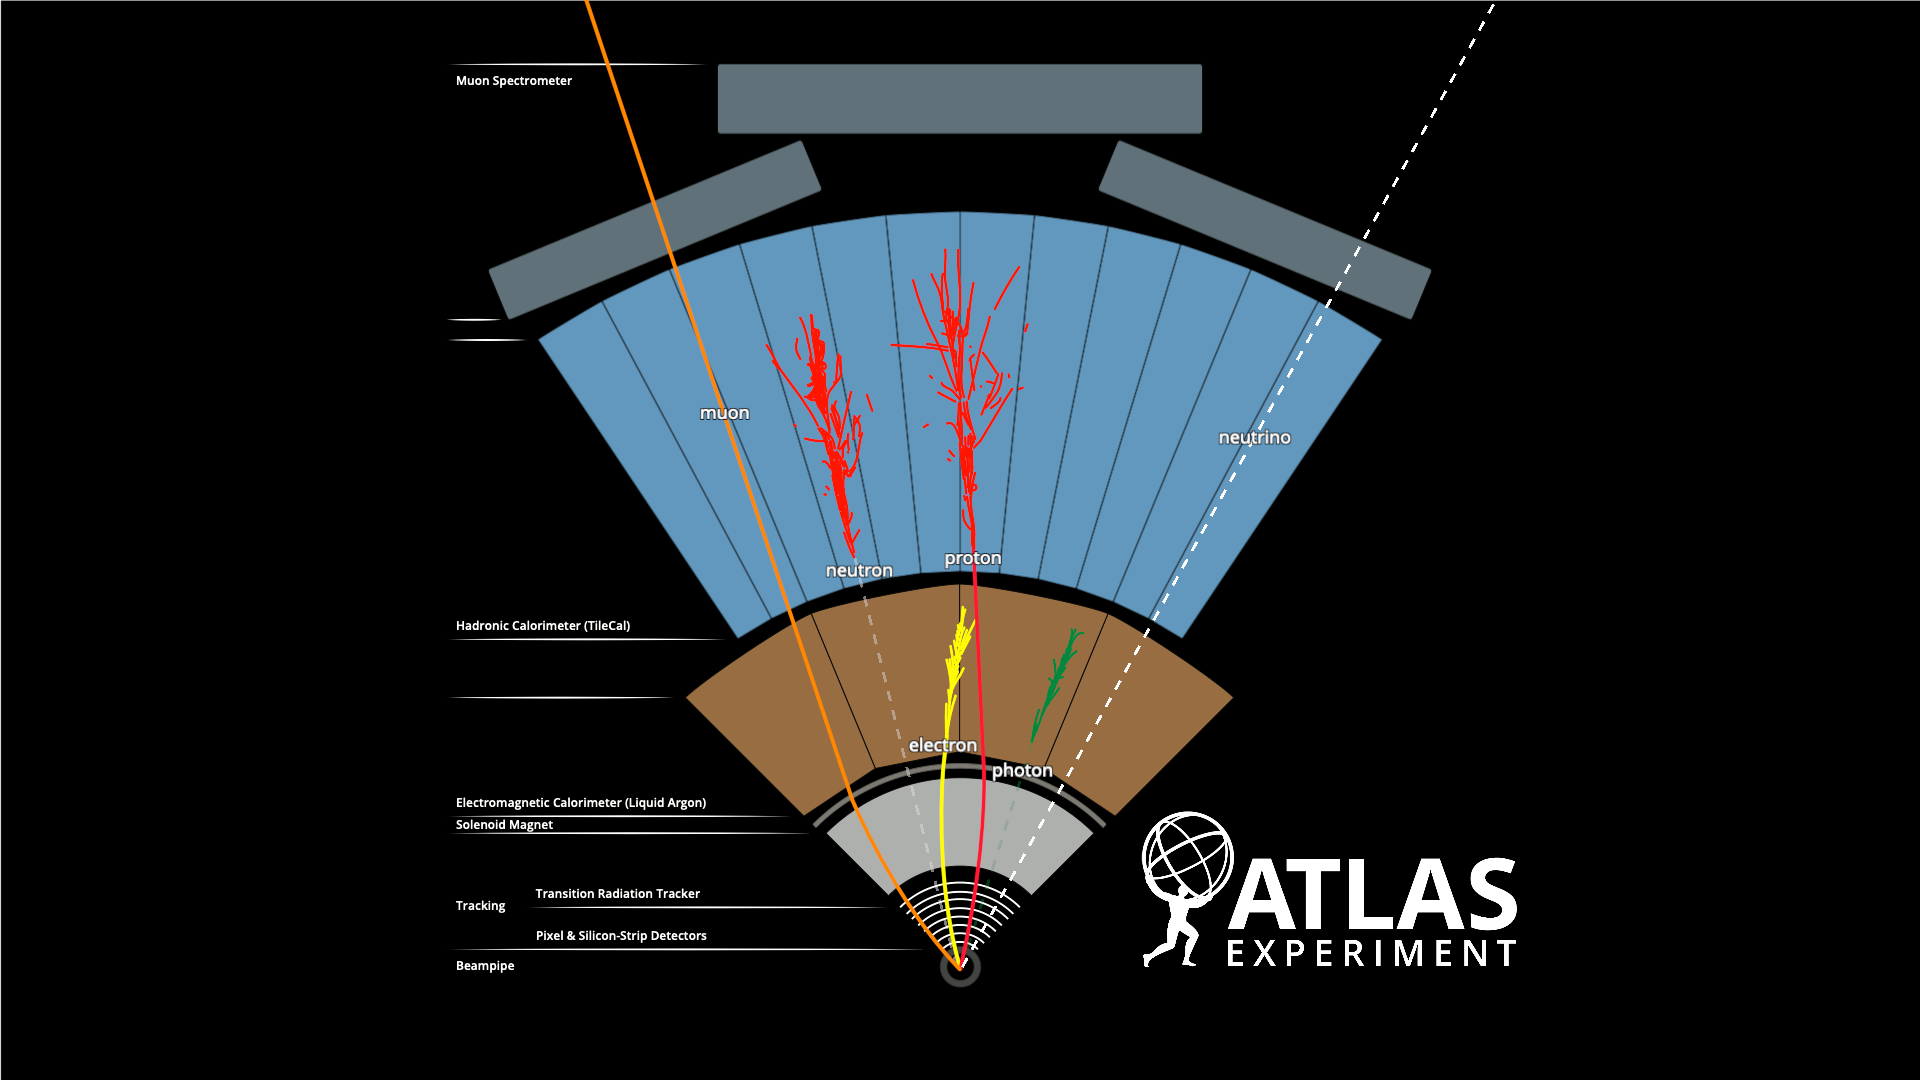
\includegraphics[width=\linewidth,height=\textheight,keepaspectratio]{reconstruction/ATLAS_Detector_Schematic_black_particles}
            \caption{
                Depiction of different particle types showering through the ATLAS detectors\cite{Mehlhase:2770815}.
            }
            \label{fig:atlas_shower}
        \end{figure}


        \subsection{Jet Definition}
            
        Jets are used to represent a range of physical phenomenon,
            from scattering within calorimeters to the process of hadronic showering.
        The general goal is to have each jet correspond to one particle/parton.
        Doing so allows energy clusters and tracks to be connected to each other
            and (ideally) reconstructed back to the final state particles produced in the interaction region.
        In practice however, particles frequently overlap in their energy deposition,
            making it challenging to distinguish where one particle should begin and another should end.
        Historically, a number of different jet algorithms have been used to describe particle showers.
        In ATLAS, the jet algorithm currently in use is the \textit{\antikt} clustering algorithm\cite{anti_kt}.
        Adoption of \antikt has been motivated by its robust ability to isolate jet boundaries both between jets
            and from the surrounding stochastic noise of the detector.
        The \antikt algorithm has a single input parameter ``$\Rparam$'' which roughly corresponds to the $\Delta R$ ``radius''
            of the jets that \antikt should attempt to match to.
        Radius here refers to the solid angle distance 
            $\Delta R^2 \equiv \Delta \eta^2 + \Delta \phi^2$.
        An $\Rparam$-parameter value of 0.4 is the standard for jets in ATLAS, and is used for this analysis.
        This value means that \antikt will generally keep aggregating cells together until the jet cluster's
            $\Delta R$ radius equals 0.4, and not much beyond that.


        \FloatBarrier
        \subsection{Jet Calibration} \label{sec:jet_calibration}

        Once jets have been formed, their energy and momentum must be calibrated.
        As discussed in Section \ref{sec:calorimeter}, the ATLAS calorimeters are sampling calorimeters.
        This means that the bulk of energy deposited is lost in inactive material and not read out.
        Additional energy losses are incurred from inefficiencies in the clustering algorithm and from the \textit{non-compensating} nature of ATLAS calorimeters.
        That is, they do not have an intrinsic method to account for the fact that electromagnetic radiation deposits a higher fraction of its energy into the detectors than hadronic radiation\cite{cell_clustering}.
        Instead, the energy that \textit{is} deposited in the calorimeters is scaled up by a correction factor,
            which was determined in advance using test particles with known parameters\cite{jet_energy_measurment}.
        These energy calibrations are done at the electromagnetic scale,
            meaning the calibration tests and factors were derived from electromagnetic particle showers.
        The calorimeters are less sensitive to hadronic showers,
            and so for these the energy correction factors are further adjusted using Monte Carlo simulation results.
        After correcting for energy, the next step is to correct for momentum.
        Reconstructed jets are assumed to originate from the hard-scatter interaction point.
        Thus, the momentum vectors associated with the jets and their topo-clusters are adjusted to point away from the PV.

        The final step in the jet reconstruction process is the track-matching algorithm.
        To improve the performance of reconstructing jet energy,
            track momentum is used to replace the measured energy of topo-clusters in jets where possible.
        This is done via an algorithm called \textit{Particle Flow},
            which first identifies tracks that can be associated with a jet.
        Particle Flow then attempts to match these associated tracks to individual topo-clusters.
        If such a match can be made, the energy of the topo-cluster is replaced with the reconstructed momentum of the matched track.
        This is done because (at low $p_T$) track momentum can be more reliably measured in ATLAS than cluster energy,
            and with such relativistic particles their momentum is effectively equivalent to their energy.
        The resulting jet-track combination objects are known as \textit{PFlow Jets},
            which are then used for the rest of the reconstruction process\cite{pflow}.

    \section{Flavor Tagging}
        
        There are many kinds of particles and processes that can produce jets.
        One particular kind of jet integral to this analysis is that of b-quark-initiated jets,
            more simply known as b-jets.
        B-jets are important because, of all the particles the Higgs can decay to,
            its branching ratio to a $\bbar$ pair is highest (Table \ref{tab:higgsbranching}).
        Distinguishing b-jets from other jet types
            (noteably, the light-jets produced from the VBF initial-scatter quarks),
            achieved through the process of \textit{flavor tagging},
            is therefore of paramount importance in this analysis.
        Flavor Tagging in ATLAS is performed in two stages;
            first with a set of simple low-level taggers based on impact parameters and secondary vertexing,
            and then with a set of more sophisticated taggers which use the low-level tagger information as inputs.


        \subsection{Impact Parameter Taggers}

            The low-level b-tagging algorithms can be divided between impact parameter taggers and secondary vertexing algorithms.
            IP2D and IP3D are the basic two and three-dimensional impact parameter-based taggers, 
                alongside RNNIP\cite{rnnip}, a recurrent neural network-based tagger (see Section \ref{sec:ml_techniques}).
            They take every track associated with a PFlow Jet
                and then use a slightly modified version of the perigee parameters discussed above in order to tag it.
            Namely, the $d_0$ and $z_0$ parameters are given a positive or negative sign to help better emphasize key characteristics of b-jets\cite{thesis_giacinto}:
            \begin{equation} \begin{split}
                \textrm{sign}_{d0} &= \textrm{sign}(\sin(\phi_{\textrm{jet}} - \phi_{\textrm{track}}) \cdot d_{0,\textrm{track}}) \\
                \textrm{sign}_{z0} &= \textrm{sign}((\eta_{\textrm{jet}} - \eta_{\textrm{track}}) \cdot z_{0,\textrm{track}})
                \,.
            \end{split} \end{equation}
            Physically, this sign convention is related to the point at which the axis of the track vector intersects
                (in a 2D plane) with the axis of the jet momentum vector. 
            Specifically, the sign corresponds to whether the \textit{vector to that intersection}
                points along (positive sign) or against (negative sign) the jet axis vector.
            See Fig. \ref{fig:ip3d_sign} for a graphical illustration of this convention.

            \begin{figure}
                \begin{subfigure}{0.48\textwidth}
                    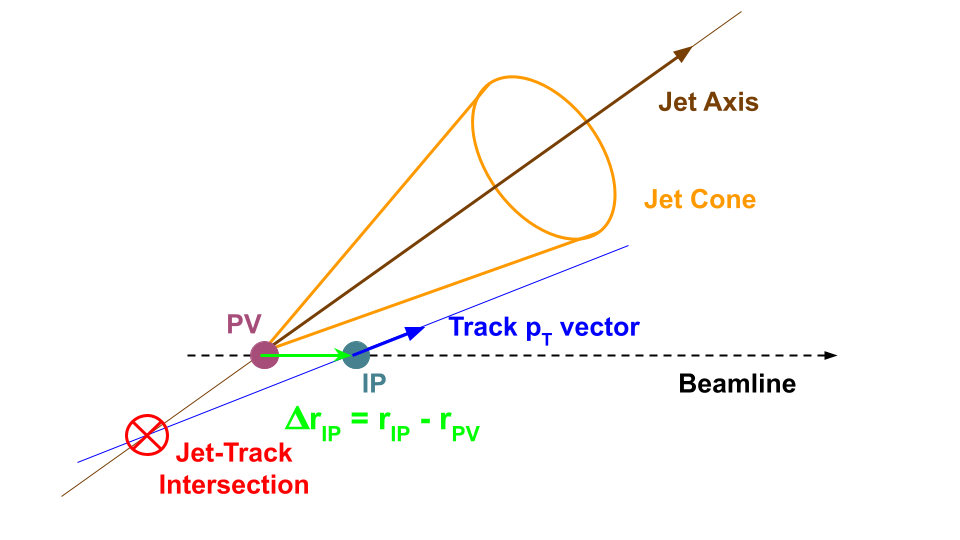
\includegraphics[width=\linewidth,height=\textheight,keepaspectratio]{reconstruction/ip3d_sign_negative}
                    \captionsetup{justification=centering} \caption{IP3D Negative Sign Convention}
                \end{subfigure}
                \begin{subfigure}{0.48\textwidth}
                    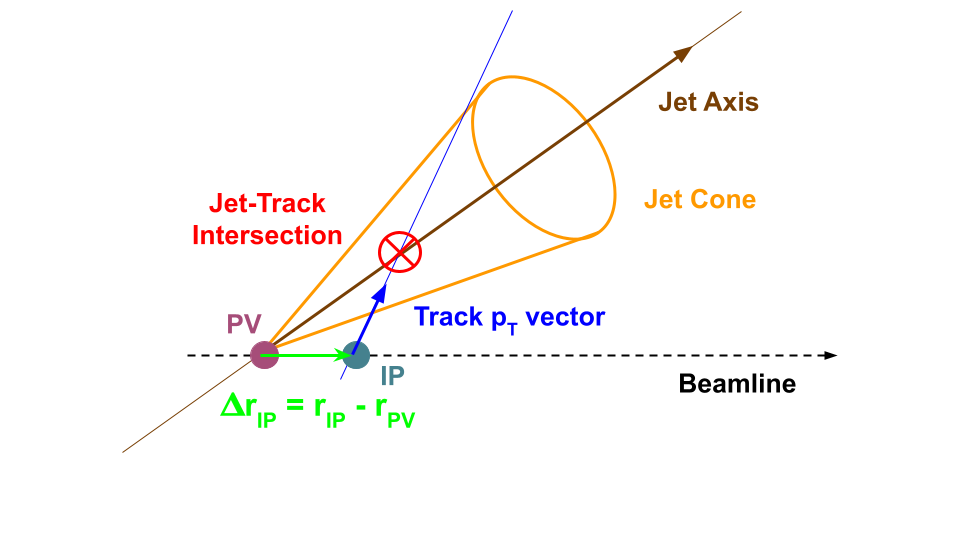
\includegraphics[width=\linewidth,height=\textheight,keepaspectratio]{reconstruction/ip3d_sign_positive}
                    \captionsetup{justification=centering} \caption{IP3D Positive Sign Convention}
                \end{subfigure}
                \caption{
                    Diagrams of the sign convention used for IP3D.
                    In the left diagram, the track $p_T$ vector intersects with the jet $p_T$ vector axis
                        \textit{before} the PV, suggesting this track originated from a source unrelated to the PV
                        (and so is likely just noise from a pileup vertex).
                    In the right diagram, the track $p_T$ vector intersects with the jet $p_T$ vector axis
                        \textit{inside} the jet (which originated from the PV),
                        suggesting this track came from a secondary vertex
                        (around the area marked with a red X)
                        of a particle originally from the PV.
                    \cite{thesis_giacinto}.
                }
                \label{fig:ip3d_sign}
            \end{figure}

            For IP2D and IP3D, values are assigned to \textit{each} track in a jet based on
                probability density functions (PDF) of the different jet types.
            Specifically, a PDF is constructed of the impact parameter \textit{significance}, $d_0/\sigma_{d0}$,
                where $\sigma_{d0}$ is the error of the measurement.
            The probability that a given track, $i$, would have some impact parameter significance value (based on the PDF)
                is that track's assigned IP2D value, $t_i$.
            IP2D and IP3D are then constructed as likelihood ratios of the product of all track-values for a jet.
            For example, the likelihood ratio of a jet being a b-jet versus a light-jet\footnote{
                    A light-jet is defined as a jet produced from the hadronization of a gluon or
                        an up, down, or strange quark.
                } would be based on the PDF of the impact parameter for
                b-jets ($\textrm{PDF}_b$) to that for light-jets ($\textrm{PDF}_l$)
            \begin{equation}
                R(t_1, t_2, ... t_N) \equiv \frac{\prod_{i=1}^N \textrm{PDF}_b(t_i)}{\prod_{i=1}^N \textrm{PDF}_l(t_i)}
                \,.
            \end{equation}
            These distributions are subsequently used as a discriminant to distinguish b-jets and charm-jets from light-jets
                (see Fig. \ref{fig:ip3dsig})\cite{thesis_giacinto}.

            \begin{figure}
                \begin{subfigure}{0.48\textwidth}
                    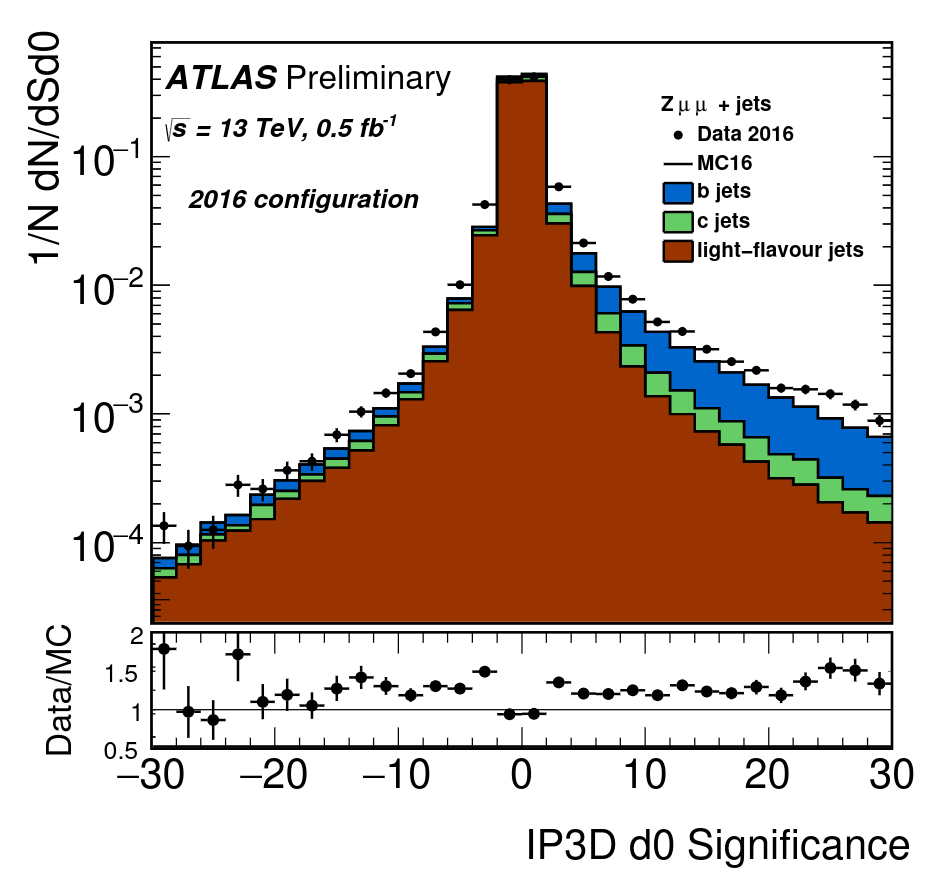
\includegraphics[width=\linewidth,height=\textheight,keepaspectratio]{reconstruction/ip3d_d0_sig_2016}
                    \captionsetup{justification=centering} \caption{IP3D-$d_0$, 2016}
                \end{subfigure}
                \begin{subfigure}{0.48\textwidth}
                    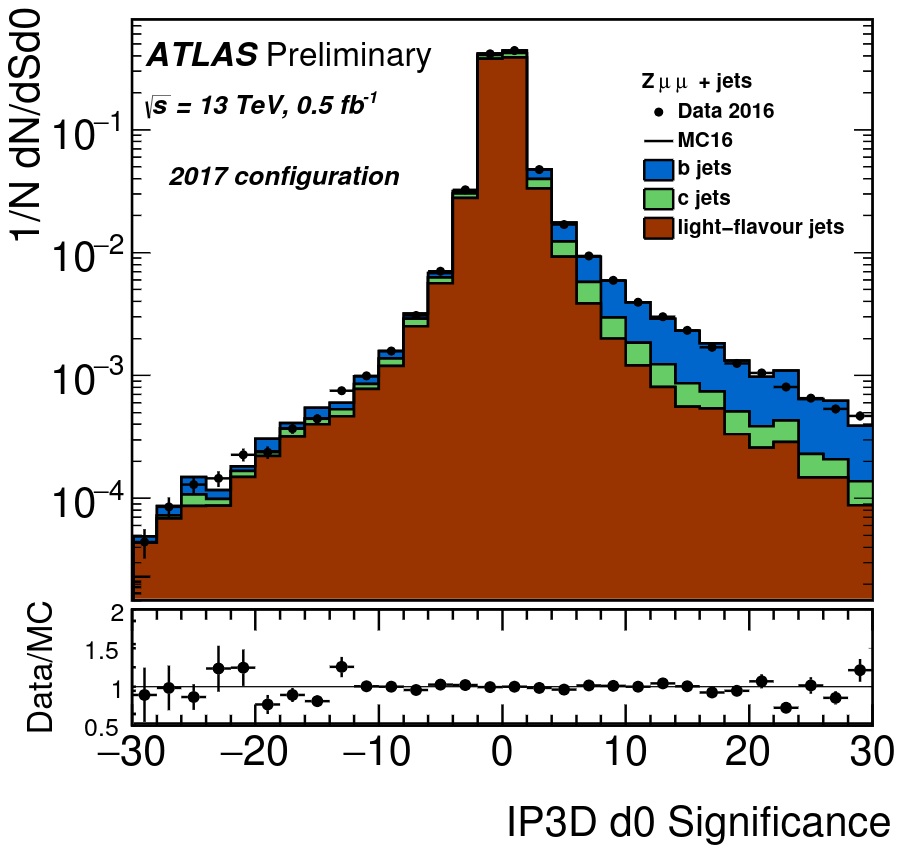
\includegraphics[width=\linewidth,height=\textheight,keepaspectratio]{reconstruction/ip3d_d0_sig_2017}
                    \captionsetup{justification=centering} \caption{IP3D-$d_0$, 2017}
                \end{subfigure} \\
                \begin{subfigure}{0.48\textwidth}
                    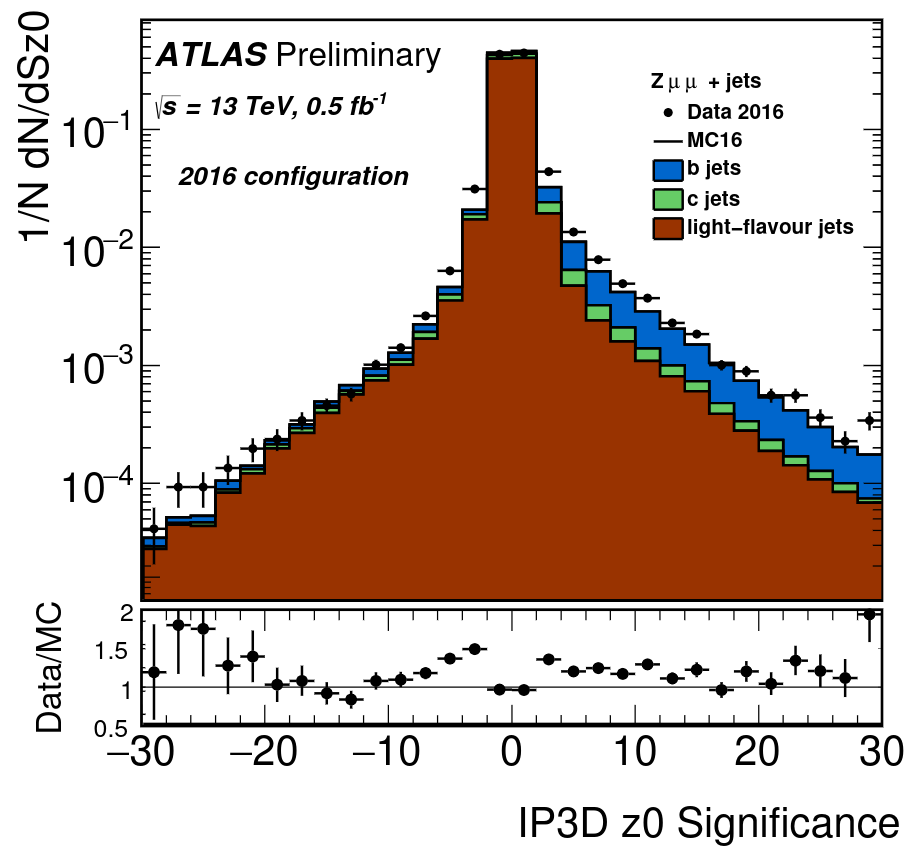
\includegraphics[width=\linewidth,height=\textheight,keepaspectratio]{reconstruction/ip3d_z0_sig_2016}
                    \captionsetup{justification=centering} \caption{IP3D-$z_0$, 2016}
                \end{subfigure}
                \begin{subfigure}{0.48\textwidth}
                    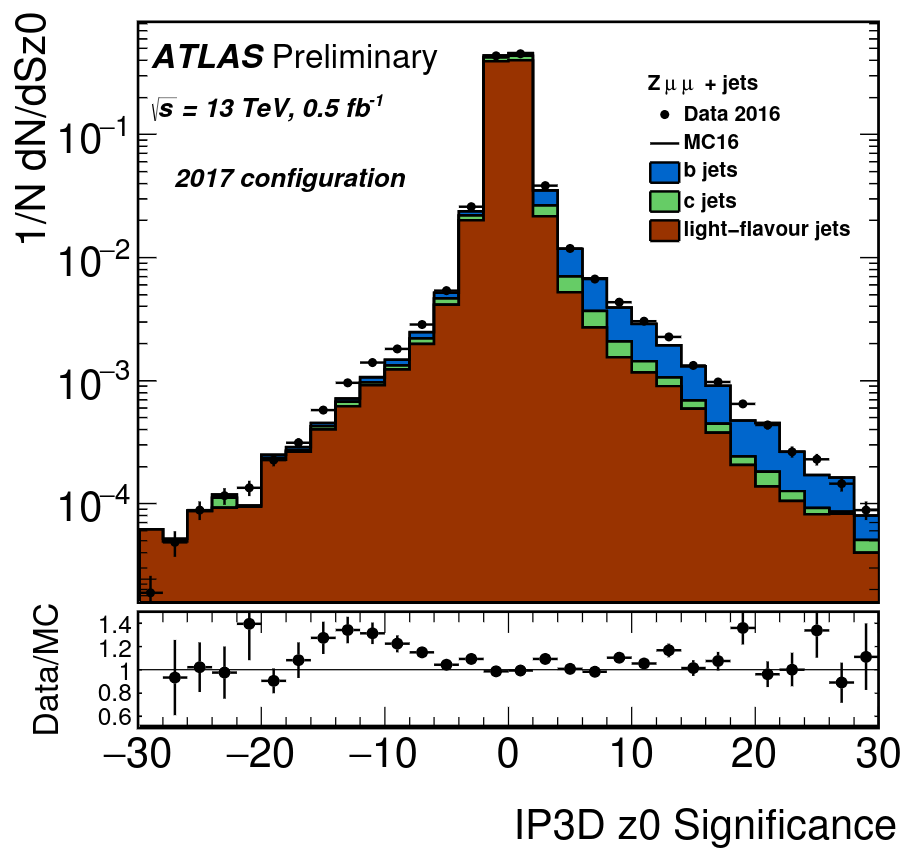
\includegraphics[width=\linewidth,height=\textheight,keepaspectratio]{reconstruction/ip3d_z0_sig_2017}
                    \captionsetup{justification=centering} \caption{IP3D-$z_0$, 2017}
                \end{subfigure}
                \caption{
                    IP3D $d_0$ and $z_0$, for 2016 and 2017 configurations of the LHC and ATLAS\cite{btagging_optimisation}.
                    Note the excess of b-jets for positive-valued IP2D and IP3D significance values as compared to charm-jets
                        and especially light-jets.
                    This excess shows how b-jets are more likely to be associated with jets possessing
                        these positive impact parameter values,
                        providing a mechanism to help identify b-jets.
                }
                \label{fig:ip3dsig}
            \end{figure}

            The IPxD taggers effectively treat all tracks in a jet as independent of each,
                combining their impact parameter information through a mere product of their LLR values.
            RNNIP, a recurrent neural network, expands upon their functionality by correlating
                the impact parameter significance values of the tracks.
            This is done by running the tagger over individual tracks sequentially
                and feeding the output of each iteration into the next as an additional input,
                allowing arbitrary numbers of tracks to be related to each other within the same jet.

            \begin{table}[tbh]
   \begin{center}
        \caption{ Inputs to IP3D and RNNIP }
        \label{tab:rnnip}
        \footnotesize
        \begin{tabular}{p{0.16\textwidth}|p{0.8\textwidth}}
        \hline
        Track Variable & Description \\
        \hline
        \hline
        & Used in IP3D and RNNIP \\
        \hline
        $S_{d0}$ &  2D impact parameter significance $d_0 / \sigma_{d0}$ \\
        $S_{z0}$ &  3D impact parameter significance $z_0 /\sigma_{z0}$\\
        Category & Based on number of observed, expected, or missing hits in silicon detectors.\\
        \hline
        \hline
        & New to RNNIP \\
        \hline
        $p_T^{\textrm{frac}}$ & The fraction of transverse momentum carried by the track relative to the jet, $p_T^{\textrm{track}} / p_T^{\textrm{jet}}$. \\
        $\Delta R$(track, jet) & The angular distance between the track and the jet axis,
            $\sqrt{(\phi_{\textrm{track}} − \phi_{\textrm{jet}} )^2 + (\eta_{\textrm{track}} − \eta_{\textrm{jet}})^2}$.\\
        \hline
        \end{tabular}
    \end{center}
\end{table}



        \FloatBarrier
        \subsection{Secondary Vertexing Algorithms}

            Secondary vertexing algorithms take advantage of the fact that b-hadrons are significantly longer lived than light-hadrons,
                and thus their associated secondary vertices typically have a larger displacement from the primary vertex.
            In ATLAS, there are two primary algorithms used to perform b-tagging with secondary vertexing.
            Realistically, hadronic matter decays in multiple steps, producing a series of close vertices each emitting more particles.
            The first of the ATLAS secondary vertex algorithms, JetFitter, seeks to reconstruct this full multi-vertex structure of the hadronic decay.
            In contrast, SV1 (Secondary Vertex 1), works by making an approximation as to how hadronic decays behave.
            SV1 takes a simpler view of the decay process, and reconstructs all the resulting tracks as products of a single secondary vertex.
            For both algorithms, several fit parameters are produced from the vertexing,
                which are then used both as discriminants themselves,
                as well as utilized in the next step as inputs to the more advanced taggers\cite{btagging_optimisation}.

        \FloatBarrier
        \subsection{High Level Taggers and Machine Learning Techniques}\label{sec:ml_techniques}

            After running all of the low-level taggers,
                the final step in flavor tagging is the use of a pair of high-level machine-learning-based tagging algorithms
                called DL1 (Deep Learning 1) and MV2 (MultiVariate tagger 2)
                \cite{bjet_id_and_performance} \cite{btagging_optimisation}.
            In order to understand how these work, it is worth taking a moment to discuss what machine learning algorithms,
                especially \textit{neural networks} are and how they operate.

            \begin{figure}[tbh] \center
                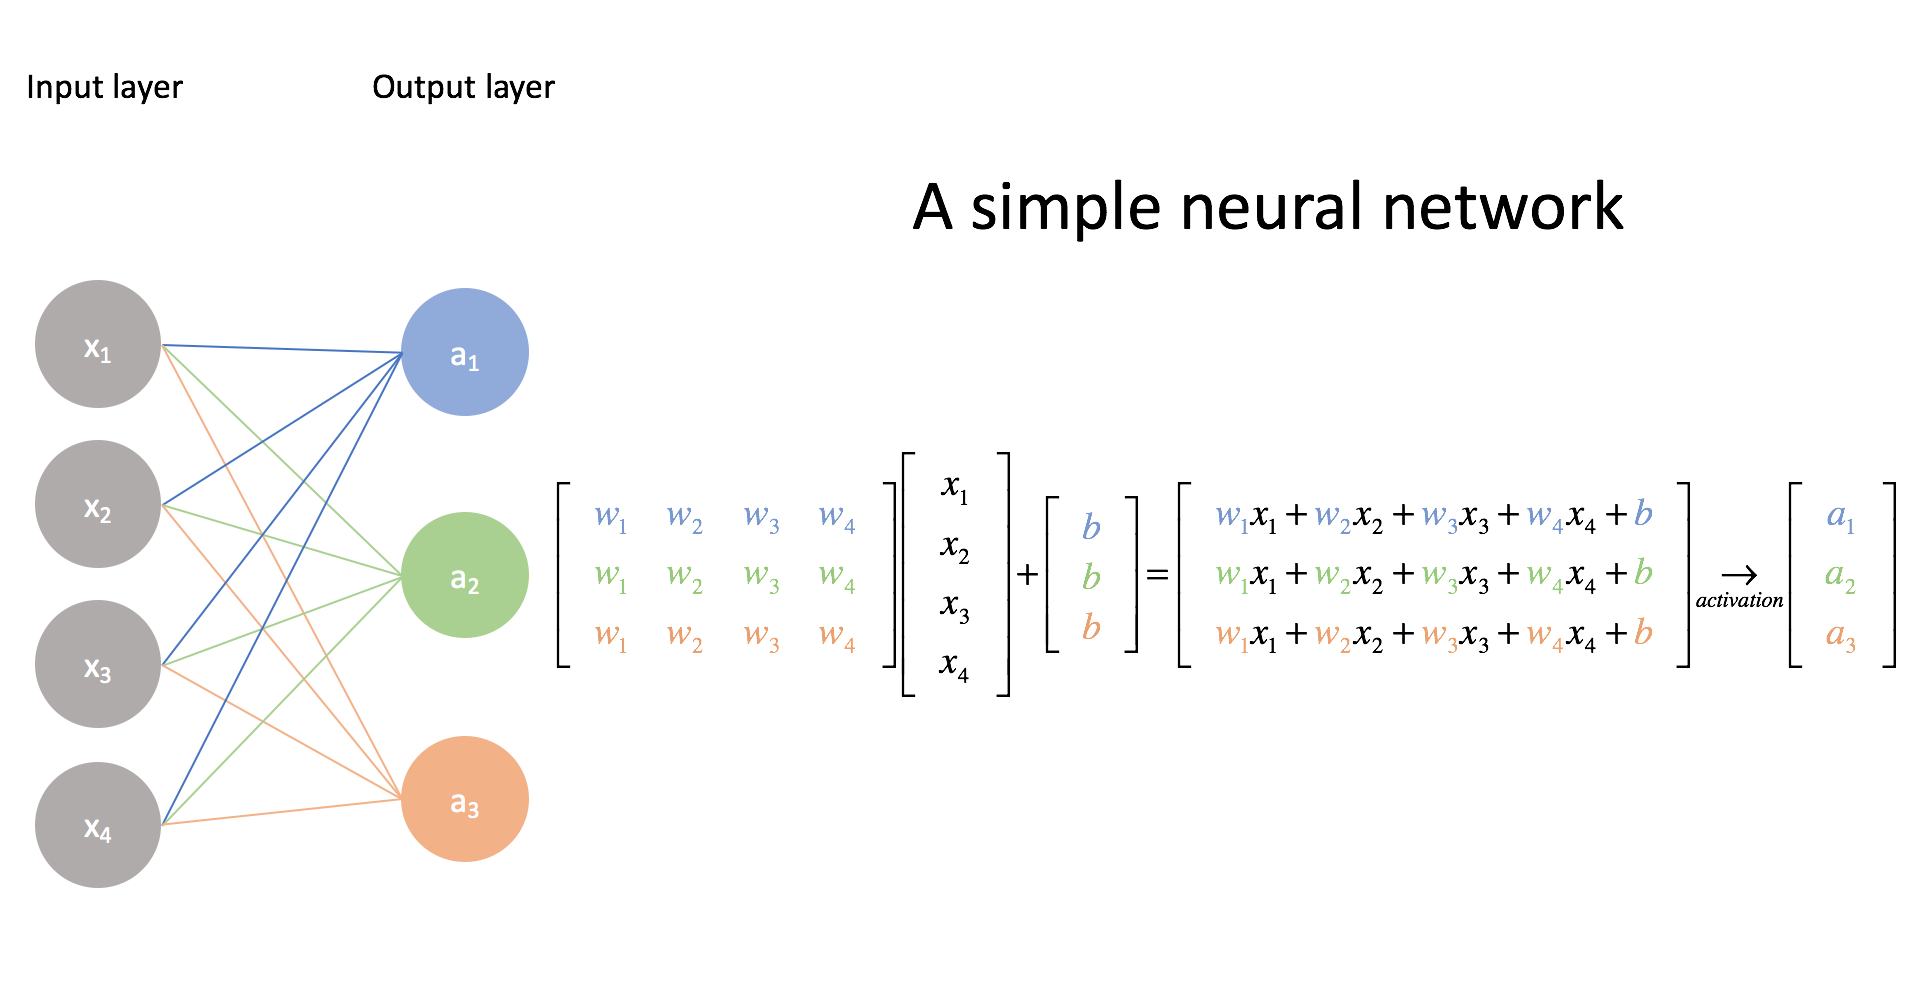
\includegraphics[width=\linewidth,height=\textheight,keepaspectratio]{reconstruction/nn_matrix}
                \caption{
                    A representation of a simple neural network \cite{intro_to_neural_networks}.
                }
                \label{fig:nn_matrix}
            \end{figure}

            A neural network at its core is a multivariable formula meant to provide some sort of discriminating metric\cite{MLatLHC}.
            For DL1 the inputs are a wide array of kinematic variables for a particular jet (Table \ref{tab:DL1_vars}).
            The output is a set of numbers specifying the tagger's confidence that a jet is
                a light, charm, or bottom jet.
            What make neural networks so powerful is how the discriminating formula is generated.
            Neural networks are arranged as a function (network) connecting the input variables to the output metrics. 
            As seen in Fig. \ref{fig:nn_matrix} this network is actually a matrix of weights,
                which is multiplied by the input layer to produce an output vector.
            Each component of the output vector is then run through some non-linear ``activation'' function\footnote{
                    For example, a sigmoid function, defined as $S(x) = \frac{1}{1+e^{-x}}$.
                } to grant the final output a more dynamic range of values than a linear function could provide.

            \begin{figure}[tbh] \center
                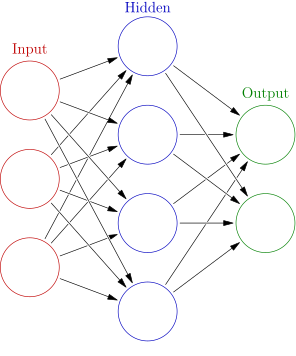
\includegraphics[width=0.5\linewidth,height=\textheight,keepaspectratio]{reconstruction/Colored_neural_network}
                \caption{
                    A representation of a neural network with a single hidden layer\cite{colored_neural_network}.
                }
                \label{fig:colored_neural_network}
            \end{figure}

            The key to the construction of a neural network is in how the weight matrix is established.
            At first the weights are random, and the network produces similarly random output that is of no use.
            However, the network undergoes an iterative training procedure, in which the weights are slightly adjusted
                and retested against a known sample of training data.
            Adjustments which lead to slightly better performance are maintained and improved upon
                with successive cycles (each cycle is referred to as an ``epoch'')
                of the training while negative adjustments are discarded.
            After enough cycles the network should ideally be tuned to provide very powerful classification.
            Of course, a trivial network such as that in Fig. \ref{fig:nn_matrix} is very limited,
                and actual neural networks typically use ``hidden layers'' between the input and output (Fig. \ref{fig:colored_neural_network}),
                with each layer corresponding to another weight matrix to be tuned by training.

            \begin{figure}
                \begin{subfigure}{0.48\textwidth}
                    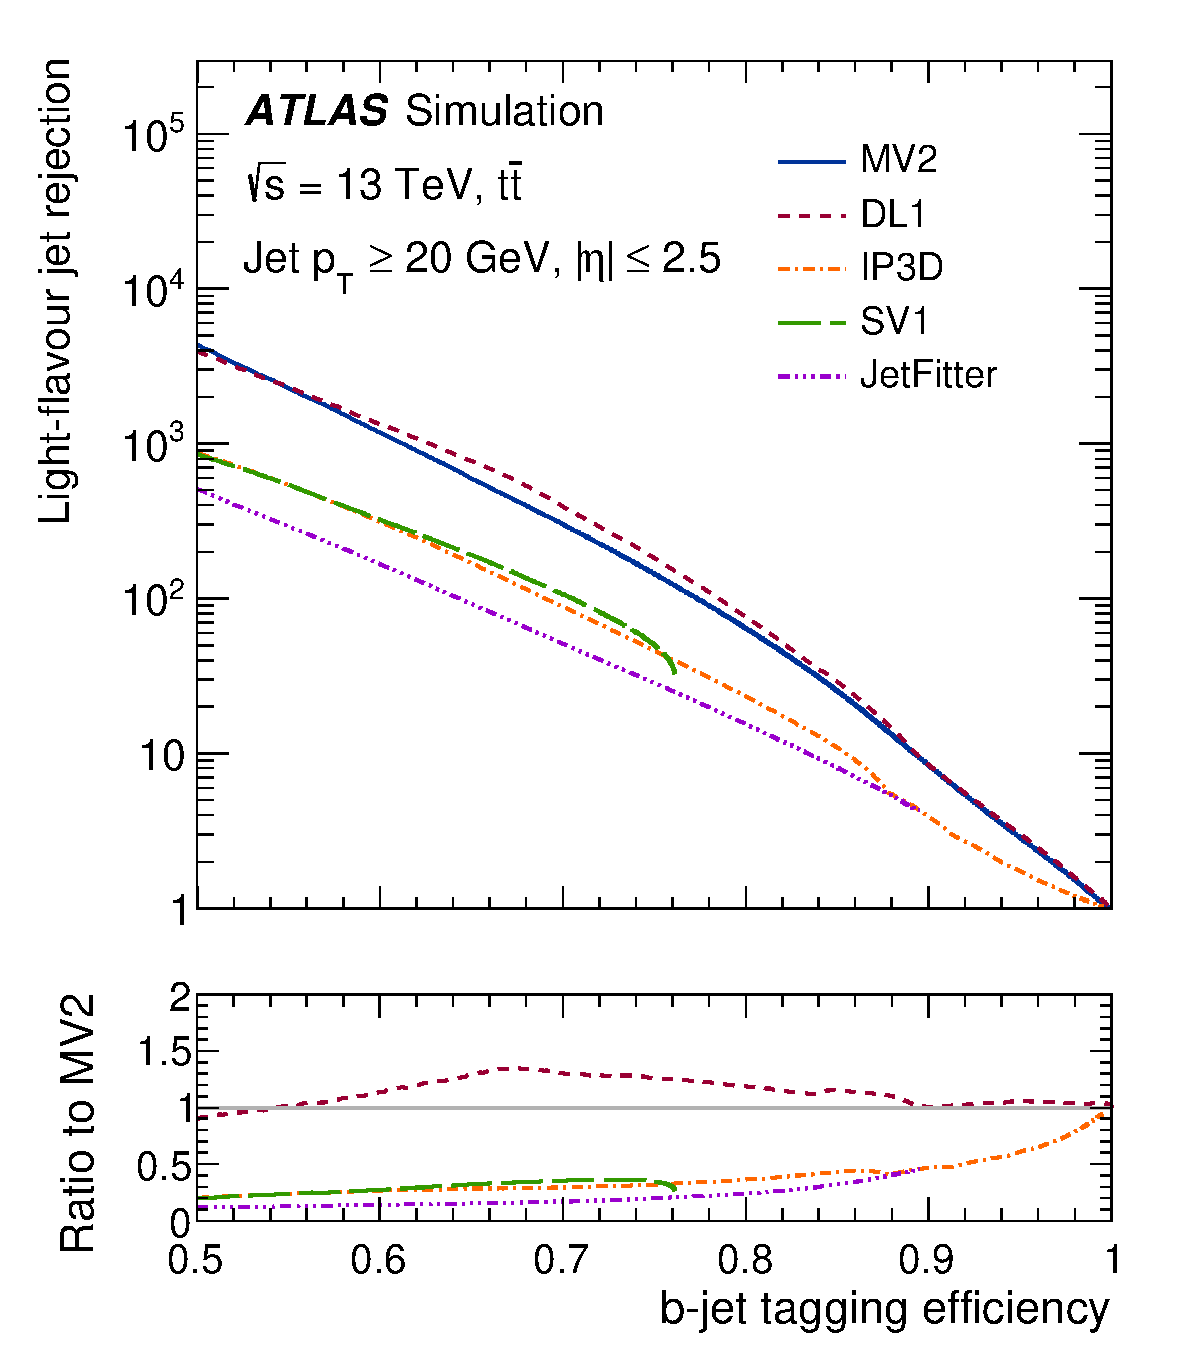
\includegraphics[width=\linewidth,height=0.35\textheight,keepaspectratio]{reconstruction/dl1_performance_ljet}
                    \captionsetup{justification=centering} \caption{Flavor Tagging Performance Against Light Jets}
                \end{subfigure}
                \begin{subfigure}{0.48\textwidth}
                    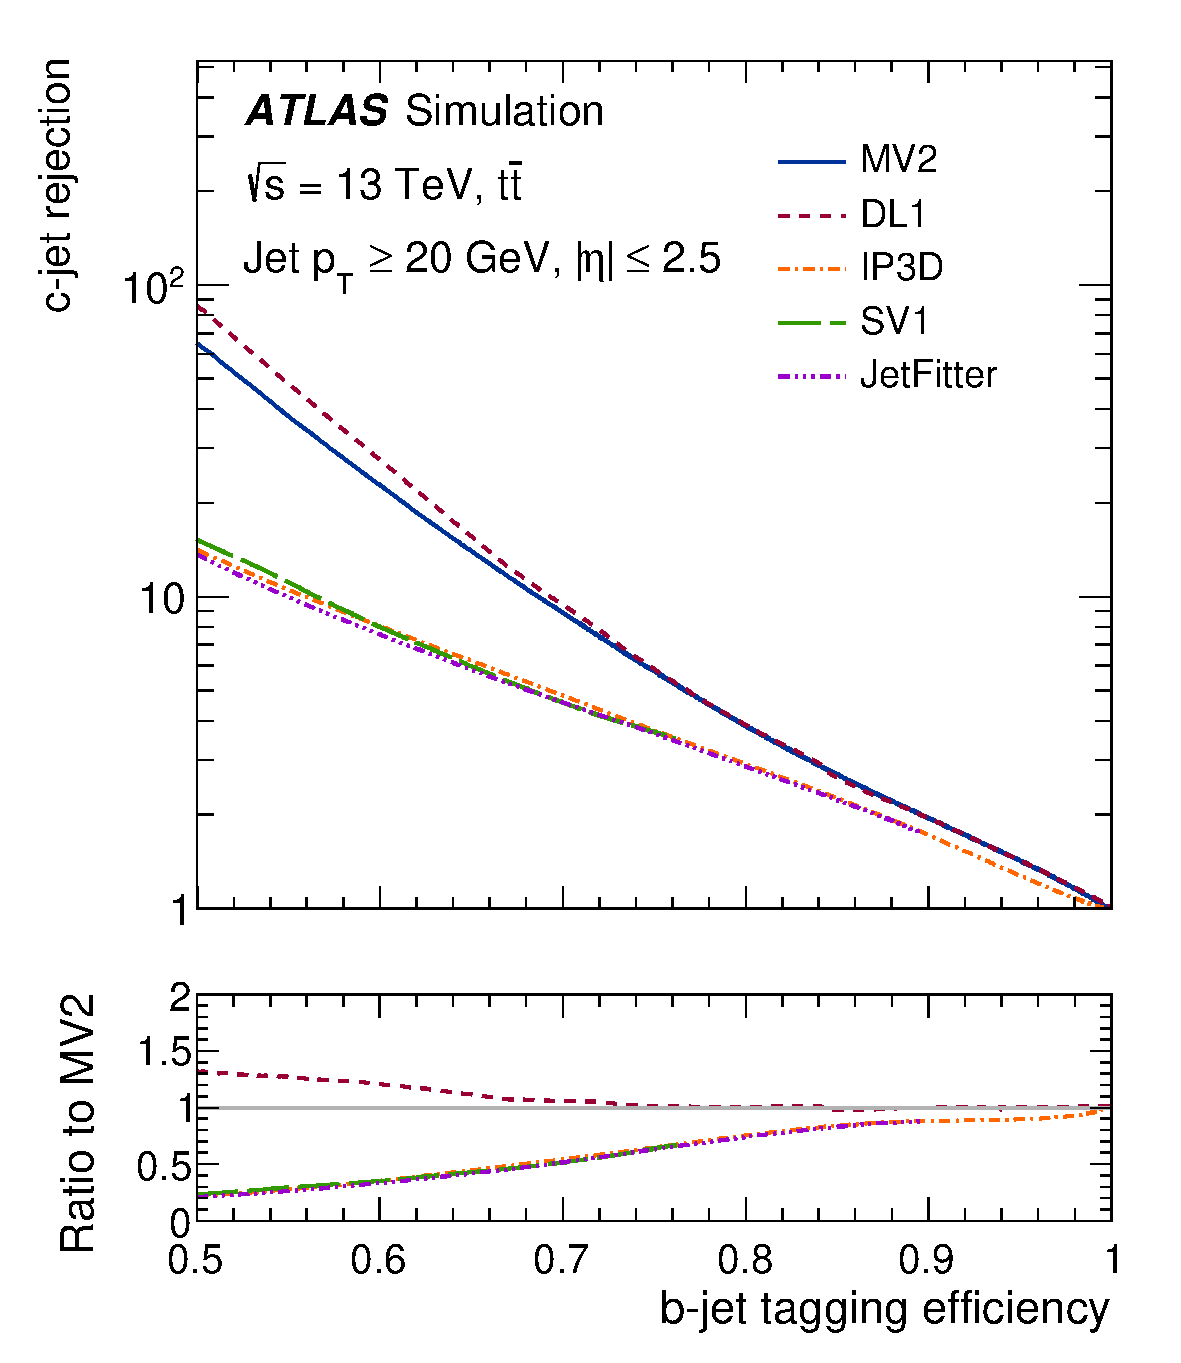
\includegraphics[width=\linewidth,height=0.35\textheight,keepaspectratio]{reconstruction/dl1_performance_cjet}
                    \captionsetup{justification=centering} \caption{Flavor Tagging Performance Against Charm Jets}
                \end{subfigure}
                \caption{
                    Plots of the various flavor taggers ability to correctly identify b-jets (efficiency, x-axis)
                        vs. their ability to correctly reject light and charm jets (purity, y-axis).
                    An efficiency score of 0.6 means 60\% of b-jets are correctly identified,
                        and a score of 1 indicates that all b-jets are accepted.
                    A light-jet rejection score of $10^3$ indicates 1 in every 1000 light jets is incorrectly identified as a b-jet,
                        and a rejection score of 1 means that all light-jets are incorrectly accepted as b-jets\cite{bjet_id_and_performance}.
                }
                \label{fig:ip3d_perf}
            \end{figure}


            Deep neural networks, like DL1, are those with multiple hidden layers.
            The ``hyperparameters'' for DL1 are shown in Table \ref{tab:DL1_hyperparams}.
            For this analysis a variation of DL1, called DL1r, is used which incorporates additional inputs from RNNIP.
        
            \begin{figure}[tbh] \center
                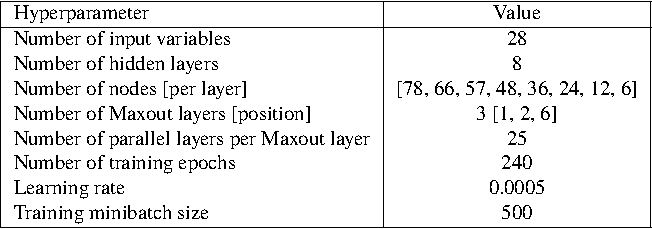
\includegraphics[width=0.7\linewidth,height=\textheight,keepaspectratio]{tables/reconstruction/DL1_hyperparams}
                \caption{
                    Hyperparameters of the DL1 neural network\cite{bjet_id_and_performance}.
                    Input variables, hidden layers, nodes, and epochs have already been discussed.
                    ``Maxout layers'' are layers in the network in which the nodes, rather than a function of their inputs,
                        are simply the maximum of the input values.
                    The ``learning rate'' controls how much the network weights are adjusted after each epoch.
                    Too low and the network will take excessively long to train,
                        but too high and the network may adjust beyond the optimal solution.
                    A ``minibatch'' is where the network training data sample is split into multiple batches and an epoch is trained over each separately.
                    The overall adjustments from the epoch are determined by combining the adjustments determined from each batch.
                }
                \label{tab:DL1_hyperparams}
            \end{figure}

            As a final note it is also worth mentioning the MV2 tagger.
            MV2 is a ``boosted decision tree,'' which is a more primitive style of machine learning.
            Decision trees undergo a similar test-and-adjust iterative training procedure to neural networks.
            However, whereas neural networks are based on a matrix arrangement,
                decision trees consist of a branching sequence of cut values that are tuned.
            Boosted decision trees like MV2 differ only in that their output is produced as an aggregate of a large number of
                separately trained trees.


            \begin{figure}[tbh] \center
                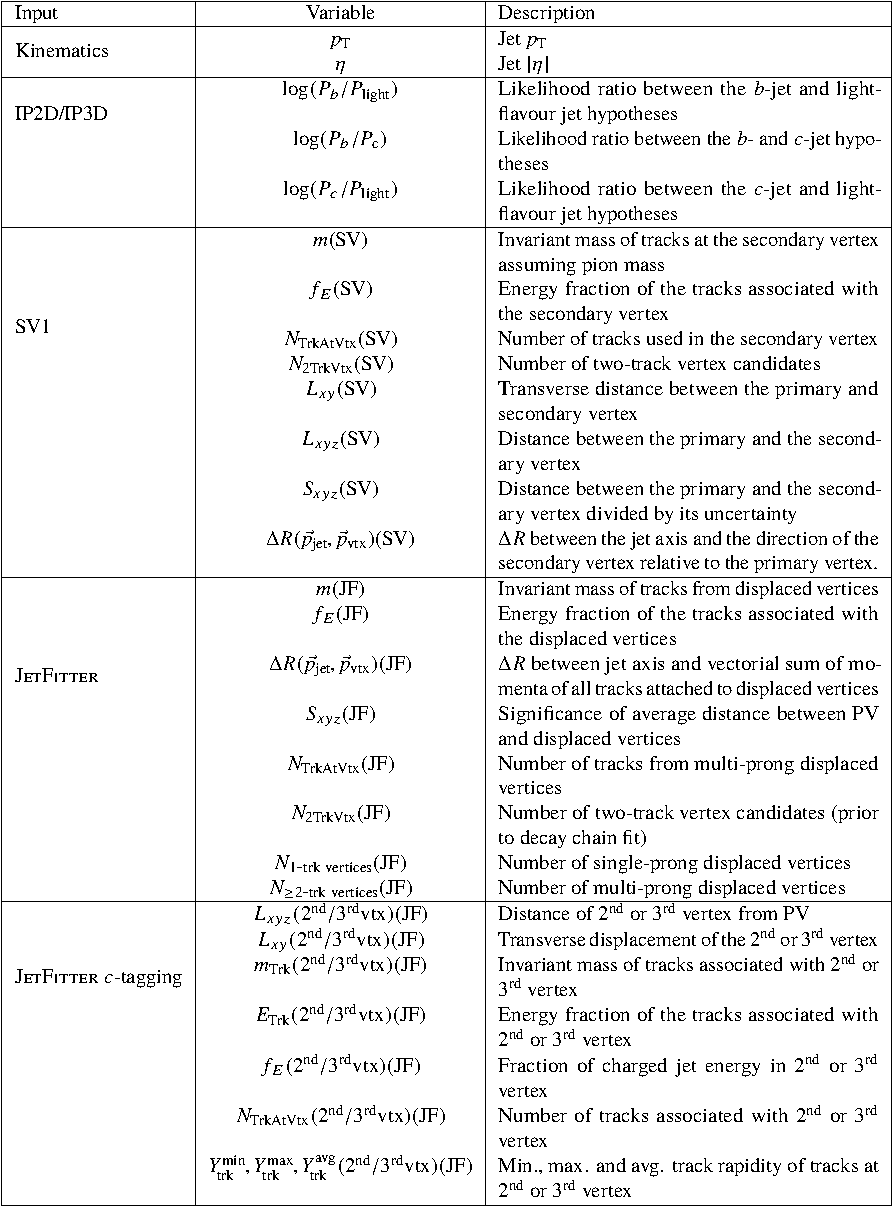
\includegraphics[width=\linewidth,height=\textheight,keepaspectratio]{tables/reconstruction/DL1_vars}
                \caption{
                    Variables used as input to DL1 and MV2 \cite{bjet_id_and_performance}.
                }
                \label{tab:DL1_vars}
            \end{figure}

    \FloatBarrier
    \section{Online vs Offline Reconstruction}

        Reconstruction is actually performed for an event twice.
        It is first done rapidly, using coarse measurements and calculations,
            for the purpose of allowing the HLT to trigger events for readout.
        These events which pass the trigger are then sent to a massive global computer cluster, called the CERN GRID.
        No longer bound by the stringent time constraints of the online running environment,
            the GRID is able to devote vast amounts of time and computing power to a second, 
            more comprehensive, reconstruction of each event.
        For both the online (HLT) and offline (GRID) environments, event reconstruction is carried out by the same suite of software,
            called \textit{Athena}\cite{athena_git}.
        The main difference in how they operate is the time they can devote to calculations, especially in the context of tracking.
        As seen is Section \ref{sec:reco_tracks}, track reconstruction is very computationally intensive.
        There are many steps, and the fitting itself is a lengthy process.
        Thus, the online environment runs a slimmed-down version of the track fitting.
        This allows the HLT to reconstruct tracks much faster, but at the expense of precision and accuracy.

        Such accuracy loss in tracking has significant downstream consequences across all aspects of reconstruction.
        Of note for this analysis are the effects on flavor tagging.
        The low-level flavor-taggers function on probability distributions of the parameters of the reconstructed tracks.
        With the degradation in track quality of the online environment, the PDFs of the low-level taggers are altered.
        Since the low-level taggers are affected, the high-level taggers are also affected.
        To account for this, the flavor tagging algorithms undergo a \textit{retuning} procedure, 
            which adjusts how the algorithms expect tracks to look.

        The retuning process operates in five steps.
        %Step1.1 - Run HLT reco on MC files;
        First, the HLT-tuned Athena framework is run on a large sample of simulation-based data,
            which emulates the reconstruction behavior of Athena in the online environment.
        %Step1.2 - Return low-level taggers on MC HLT reco;
        Based on this simulated reconstruction, the distributions used by the low-level taggers
            (e.g.\ $d_0$-significance) are recorded and turned into PDFs.
        This constitutes the retuning of the low-level taggers.
        %Step2   - Rerun HLT reco on MC, now with retuned low-level tagging info;
        With the low-level taggers retuned, the Athena reconstruction is run again,
            this time recording the output of the low-level taggers themselves.
        %Step3.1 - Perform BDT training for MV2 on HLT MC reco w/ low-level tags;
        The low-level tagger output is now fed as input to the training frameworks for the high-level taggers.
        For MV2, this is ROOT's TMVA\cite{cern_root_tmva},
            and for DL1 this is the Python package Keras\cite{keras}.
        %Step3.2 - Convert training output to usable histograms;
        Once training is complete, the output machine-learning structure is converted into a form usable by Athena,
            and the full retuning is completed.
        %Step4   - Rerun HLT reco on MC once more, to get full retuned tagging output. Use output performance to determine working points;
        At this stage, the framework is run once more, in its entirety,
            so its performance can be analyzed and any potential issues addressed.

        \begin{figure}[tbh]
            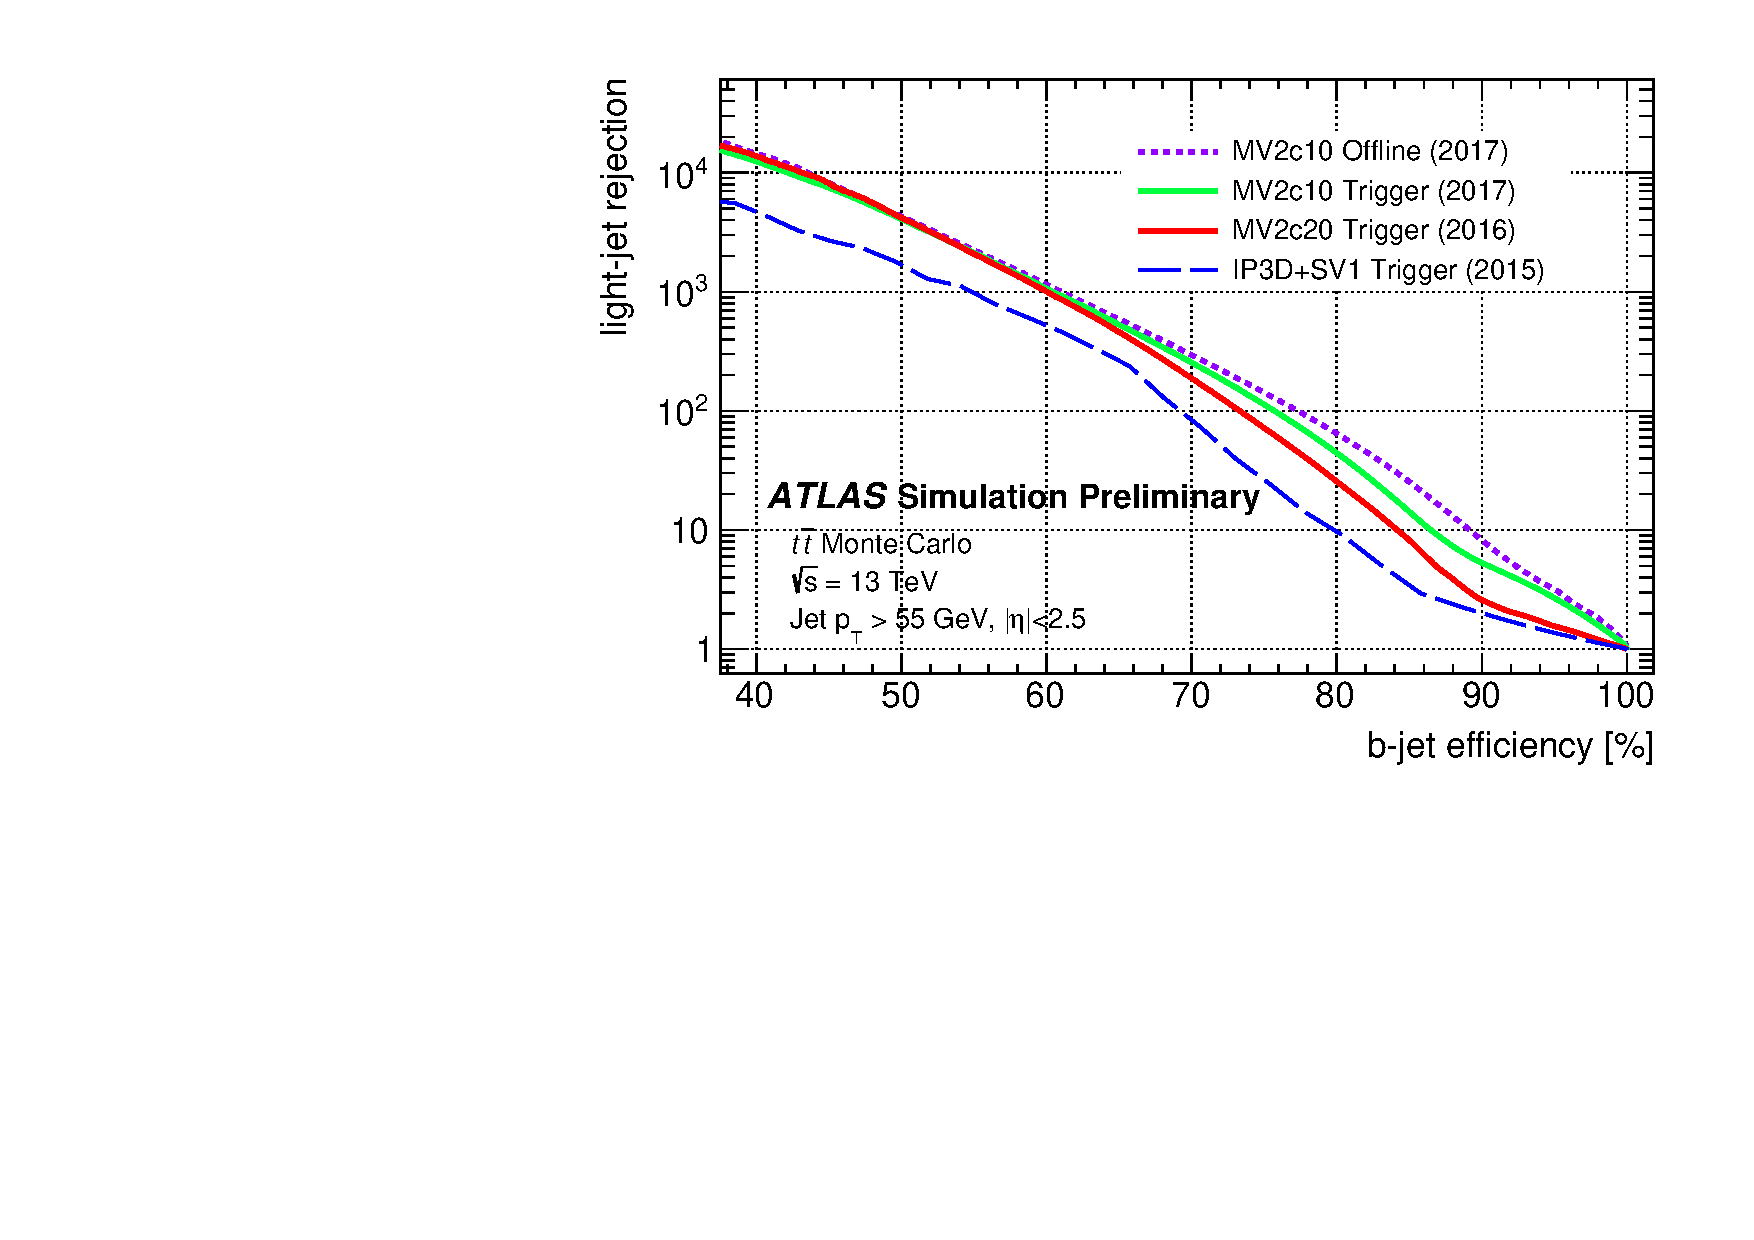
\includegraphics[width=\linewidth,height=\textheight,keepaspectratio]{reconstruction/mv2_on-off_performance}
            \caption{
                Comparison of the performance of MV2c10 and low-level taggers VS offline performance\cite{Gupta:2271945}.
                Note hat the online performance (with its lower quality tracks) is able to perform within $\approx 20\%$
                    of its offline conterpart, a remarkable improvement from the the state of MV2 earlier in Run 2.
            }
            \label{fig:mv2_performance}
        \end{figure}

        %(We don't use mv2 for the late-stage b-tag requirement on the higgs decay candidates,
        %    but we DO use it in the triggers):

